\documentclass[aspectratio=169]{beamer}

\mode<presentation>
{
  \setbeamertemplate{background canvas}[square]
  \pgfdeclareimage[width=6em,interpolate=true]{dsailogo}{../dsai-logo}
  \pgfdeclareimage[width=6em,interpolate=true]{erasmuslogo}{../erasmus-logo}
  \titlegraphic{\pgfuseimage{dsailogo} \hspace{0.2in} \pgfuseimage{erasmuslogo}}
  %\usetheme{default}
  \usetheme{Madrid}
  \usecolortheme{rose}
  \usefonttheme[onlysmall]{structurebold}
}

\usepackage{pgf,pgfarrows,pgfnodes,pgfautomata,pgfheaps,pgfshade}
\usepackage{amsmath,amssymb}
\usepackage{graphics}
\usepackage{ragged2e}
\usepackage[latin1]{inputenc}
\usepackage{colortbl}
\usepackage[absolute,overlay]{textpos}
\setlength{\TPHorizModule}{30mm}
\setlength{\TPVertModule}{\TPHorizModule}
\textblockorigin{10mm}{10mm}
\usepackage[english]{babel}
\usepackage{listings}
\setbeamercovered{dynamic}

\AtBeginSection[]{
  \begin{frame}<beamer>
  \frametitle{Outline}
  \tableofcontents[currentsection]
  \end{frame}
}

\title[Computer Vision]{Computer Vision\\Visual Odometry and SLAM}
\author{dsai.asia}
\institute[]{Asia Data Science and Artificial Intelligence Master's Program}
\date{}

% My math definitions

\renewcommand{\vec}[1]{\boldsymbol{#1}}
\newcommand{\mat}[1]{\mathtt{#1}}
\newcommand{\ten}[1]{\mathcal{#1}}
\newcommand{\crossmat}[1]{\begin{bmatrix} #1 \end{bmatrix}_{\times}}
\renewcommand{\null}[1]{{\cal N}(#1)}
\newcommand{\class}[1]{{\cal C}_{#1}}
\def\Rset{\mathbb{R}}
\def\Pset{\mathbb{P}}
\DeclareMathOperator*{\argmin}{argmin}
\DeclareMathOperator*{\argmax}{argmax}
\DeclareMathOperator*{\sign}{sign}
\def\norm{\mbox{$\cal{N}$}}
\DeclareMathOperator*{\opemin}{min}
\newcommand{\lse}{\mathfrak{se}}
\newcommand{\lso}{\mathfrak{so}}
\newcommand{\lsim}{\mathfrak{sim}}


\newcommand{\stereotype}[1]{\guillemotleft{{#1}}\guillemotright}

%\newcommand{\myfig}[3]{\centerline{\includegraphics[width={#1}]{{#2}}}
%  \centerline{\scriptsize #3}}

\newcommand{\myfig}[3]{\centerline{\includegraphics[width={#1}]{#2}}
    \centerline{\scriptsize \begin{minipage}{#1} \centering #3 \end{minipage}}}

\begin{document}

%%%%%%%%%%%%%%%%%%%%%%%%%%%%%%%%%%%%%%%%%%%%%%%%%%%%%%%%%%%%
%%             CONTENTS START HERE

%\setbeamertemplate{navigation symbols}{}

\frame{\titlepage}

%--------------------------------------------------------------------
%\part<presentation>{Part name}
%
%\frame{\partpage}

%\begin{frame}
%\frametitle{Readings}

%Readings for these lecture notes:
%\begin{itemize}
%\item[-] Russell and Norvig, Chapter 15
%\item[-] Moon and Stirling, Chapter 13
%\item[-] Forsyth and Ponce, Chapter 17
%\item[-] Isard and Blake, 1998
%\end{itemize}

%These notes contain material $\copyright$ Russell and Norvig, 2003;
%Isard and Blake, 1998; Moon and Stirling, 2000; Forsyth and Ponce,
%2001.

%\end{frame}


%--------------------------------------------------------------------
\section{Introduction}
%--------------------------------------------------------------------

\begin{frame}
\frametitle{Introduction}
\framesubtitle{Recursive state estimation}

\alert{Tracking} means doing recursive \alert{state estimation} of
a system over time using \alert{discrete, noisy observations}.

\begin{block}{Examples of system states we might want to track:}
\begin{enumerate}
\item $x,y,z,\dot{x},\dot{y},\dot{z}$ of a hostile airplane or
  missile
\item $x,y,z,\phi,\rho,\theta$ of a camera on a moving robot
\item $x,y,\theta,\dot{x},\dot{y},\dot{\theta}$ of a robot on a
  football field
\item 27 degrees of freedom of a model of the human hand
\item $x,y,z$ positions of Mercury, Venus, Earth, Mars, Jupiter, Saturn,
    Neptune, Pluto
\end{enumerate}
\end{block}

\end{frame}

%--------------------------------------------------------------------
\begin{frame}
\frametitle{Introduction}
\framesubtitle{Noisy measurements}

\begin{block}{Examples of noisy measurements helpful for state estimation:}
\begin{enumerate}
\item Angular rotation of a radar rig when the missile is detected
\item Robot-relative pitch and yaw of 3 known landmarks
\item $x,y,\theta$ of the robot measured from an image
\item Center of gravity and fingertip positions in an image of the hand
\item Pitch and yaw of the planets at particular times, relative to
  Kepler's house in Prague
\end{enumerate}
\end{block}

\medskip

Many methods exist, but the \alert{Kalman filter} (Kalman, 1960) is
the most widely used.

\end{frame}

%--------------------------------------------------------------------

\begin{frame}
\frametitle{Introduction}
\framesubtitle{Notation}

We'll use the following notation in these lecture notes:
\begin{itemize}
\item Both probability densities and discrete probability
distributions are written $P(\cdot)$.
\item Vectors are written in bold face (e.g.\ $\vec{x}$) and scalars
  are written in italics (e.g.\ $x$).
\item Random variables are written in uppercase (e.g.\ $P(\vec{X}) =
  \norm( \vec{\mu}, \Sigma )$).
\item Particular values of a random variable are written in lowercase
  (e.g.\ $P(\vec{X}=\vec{x} \mid \vec{Y}=\vec{y}) \propto e^{
  -\frac{1}{2} (\vec{x}-\vec{y}) \Sigma^{-1} (\vec{x}-\vec{y})}$).
\item $P(\vec{x})$ is shorthand for $P(\vec{X}=\vec{x})$.
\end{itemize}
\end{frame}

%--------------------------------------------------------------------
\section{The Kalman filter}
%--------------------------------------------------------------------

\begin{frame}
\frametitle{The Kalman filter}
\framesubtitle{The setting}

\begin{block}{Kalman filter assumptions}
\begin{itemize}
\item Time is \alert{discrete}.
\item The state vector $\vec{x}_{t+1}$ at time $t+1$ is a
  \alert{linear} function of the state $\vec{x}_t$ at time $t$, with
  noise added.
\item We have a linear \alert{sensor} producing at each time $t$ a
  noisy \alert{observation} of the system's state.
\end{itemize}
\end{block}

Then tracking means estimating, at every time $t$, the mean
$\vec{\mu}_t$ and covariance $\Sigma_t$ of a $d$-dimensional Gaussian
distribution $P(\vec{X}_t\mid \vec{z}_{1:t})$.

\medskip

Kalman filtering works in two steps:
\begin{enumerate}
\item \alert{Prediction} of the state $\vec{x}_{t+1}$ using
  $\vec{\mu}_t$ and the \alert{transition model}.
\item \alert{Updating} the state estimate $\vec{\mu}_{t+1},
  \Sigma_{t+1}$ using the prediction and the \alert{observation}
  $\vec{z}_{t+1}$.
\end{enumerate}
\end{frame}

%--------------------------------------------------------------------
\begin{frame}
\frametitle{The Kalman filter}
\framesubtitle{State prediction}

Suppose we have a state estimate $P(\vec{X}_t \mid \vec{z}_{1:t})$ for time
$t$ and a transition model $P(\vec{X}_{t+1} \mid \vec{x}_t)$.

\medskip
\alert{Conditioning} on $\vec{x}_t$,
we can then predict the state at time $t+1$ as
\[ P(\vec{X}_{t+1} \mid \vec{z}_{1:t}) = \int_{\vec{x}_t}
     P(\vec{X}_{t+1} \mid \vec{x}_t) P(\vec{x}_t|\vec{z}_{1:t})
     d\vec{x}_t \]

If $ P(\vec{X}_{t+1} \mid \vec{x}_t)$ and $P(\vec{X}_t|\vec{z}_{1:t})$
are both Gaussian, we have a convolution of two Gaussians, which will
always be another Gaussian.

\medskip
If we ignore the observations and just predict forward in time, we
begin with the prior $P(\vec{X}_0) =
\norm(\vec{\mu}_0,\Sigma_0)$ then predicting forward we
always have a spreading Gaussian state distribution.

\end{frame}

%--------------------------------------------------------------------
\begin{frame}
\frametitle{The Kalman filter}
\framesubtitle{Example in one dimension}

Consider a \alert{random walk} of a continuous state variable $X_t$
and a noisy observation $Z_t$.

\medskip
Perhaps you track your roommate's ``happiness'' using a happiness
survey or facial expression
measurement sensor administered once per day,
converted into a scalar index.
Without knowing the underlying factors influencing happiness, we
simply assume a random walk.

\medskip
We begin with the \alert{prior} distribution over $X_0$, i.e.,
\[ P(x_0) = \alpha e^{ - \frac{(x_0-\mu_0)^2}{2 \sigma_0^2}
  } \]

\end{frame}

%--------------------------------------------------------------------
\begin{frame}
\frametitle{The Kalman filter}
\framesubtitle{Example in one dimension}

The transition model just adds a random perturbance with variance
$\sigma_x^2$:
\[ P(x_{t+1} \mid x_t) = \alpha e^{ - \frac{(x_{t+1}-x_t)^2}{2\sigma_x^2} } \]

\medskip

Now consider what happens when we predict $X_1$ from $P(X_0)$:
\begin{eqnarray*}
P(x_1) & = & \int_{-\infty}^{\infty} P(x_1|x_0) P(x_0) dx_0 \\
       & = & \alpha \int_{-\infty}^{\infty} e^{-
               \frac{(x_1-x_0)^2}{2\sigma_x^2} }
             e^{-\frac{(x_0-\mu_0)^2}{2\sigma_0^2} } dx_0 \\
       & = & \alpha \int_{-\infty}^{\infty} e^{-
         \frac{\sigma_0^2(x_1-x_0)^2 +
         \sigma_x^2(x_0-\mu_0)^2}{2\sigma_0^2\sigma_x^2}} dx_0 .
\end{eqnarray*}
\end{frame}

%--------------------------------------------------------------------
\begin{frame}
\frametitle{The Kalman filter}
\framesubtitle{Example in one dimension}

Note that the numerator inside the exponential is quadatic in $x_0$.
We can complete the square using the equation
\[ ax_0^2 + bx_0 + c = a \left( x_0 - \frac{-b}{2a} \right)^2 +
  c - \frac{b^2}{4a} \]
giving
\[ P(x_1) = \alpha e^{ -\frac{1}{2} \left( c - \frac{b^2}{4a}
         \right)} \int_{-\infty}^{\infty} e^{ - \frac{a}{2}
         \left( x_0 - \frac{-b}{2a}\right)^2} dx_0 .
\]
but the intergral is now over the full range of a Gaussian, which is
constant, so we finally obtain, after simplification,
\[ P(x_1) = \alpha e^{ -\frac{1}{2} \left(
         \frac{(x_1-\mu_0)^2}{\sigma_0^2 + \sigma_x^2} \right)}. \] We
have a new Gaussian with mean $\mu_0$ and variance
$\sigma_0^2+\sigma_x^2$.

\end{frame}

%--------------------------------------------------------------------
\begin{frame}
\frametitle{The Kalman filter}
\framesubtitle{Example in one dimension}

After computing the \alert{prediction} $P(X_1)$, we need to
\alert{update}, incorporating the observation $z_1$.

\medskip
Now we have (using Bayes' rule)
\begin{eqnarray*}
P(x_1 \mid z_1) & = & \alpha P(z_1 \mid x_1) P(x_1) \\
                & = & \alpha e^{
                -\frac{(z_1-x_1)^2}{2\sigma_z^2} } e^{
                -\frac{(x_1-\mu_0)^2}{2(\sigma_0^2+\sigma_x^2)}
                }
\end{eqnarray*}
Completing the square and simplifying, we can obtain a Gaussian with
mean and variance
\begin{eqnarray*}
\mu_{t+1} & = & \frac{( \sigma_t^2 + \sigma_x^2 ) z_{t+1} + \sigma_z^2
\mu_t}{ \sigma_t^2 + \sigma_x^2 + \sigma_z^2 } \\
\sigma_{t+1}^2 & = & \frac{(\sigma_t^2 + \sigma_x^2)\sigma_z^2}{\sigma_t^2
+ \sigma_x^2+\sigma_z^2}
\end{eqnarray*}

\end{frame}


%--------------------------------------------------------------------
\begin{frame}
\frametitle{The Kalman filter}
\framesubtitle{Example in one dimension}

\begin{columns}
\column{5cm}

What happens when $\sigma_0=1.0$, $\sigma_x=2.0,$
$\sigma_z=1.0$, and $z_1=2.5$?

\medskip
$P(X_1)$ (the prediction) is a Gaussian with mean 0 and variance
$\sigma_0^2+\sigma_x^2$.

\medskip
$P(X_1 \mid z_1)$ (the updated state estimate) is a Gaussian with mean
$\frac{(\sigma_0^2+\sigma_x^2)z_1+\sigma_z^2\mu_0}
{\sigma_0^2+\sigma_x^2+\sigma_z^2} = 2.08$ and variance
$\frac{(\sigma_0^2+\sigma_x^2)\sigma_z^2}
{\sigma_0^2+\sigma_x^2+\sigma_z^2}=0.83$

\column{6cm}
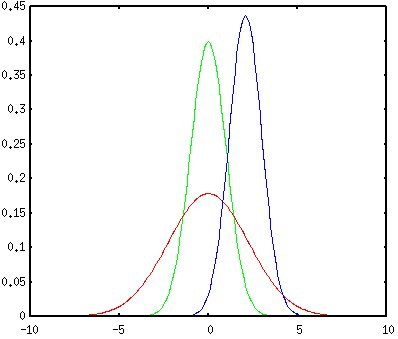
\includegraphics[width=6cm]{kalman-fig.jpg}
\end{columns}

\begin{textblock}{3}(2.35,0.9)
$P(X_0)$
\end{textblock}
\begin{textblock}{3}(2.25,1.5)
$P(X_1)$
\end{textblock}
\begin{textblock}{3}(3.05,0.8)
$P(X_1 \mid z_1)$
\end{textblock}

\end{frame}

%--------------------------------------------------------------------
\begin{frame}
\frametitle{The Kalman filter}
\framesubtitle{Example in one dimension}

\begin{block}{Observations about the 1D Kalman update}
\begin{itemize}
\item After predicting we are \alert{less confident} in our state estimate.
\item When the observation arrives, our new estimate is a
      \alert{weighted mean} between the observation and the prediction.
\item The variance $\sigma_t$ does not depend on $z$, so if $\sigma_z$
      and $\sigma_x$ never change, $\sigma_t$ will converge to a fixed
      value over time.\end{itemize}
\end{block}

\end{frame}

\begin{frame}
\frametitle{The Kalman filter}
\framesubtitle{General Kalman filter system model}

In general we have a multivariate Gaussian
\[ \norm(\vec{\mu},\mat{\Sigma})(\vec{x}) = \alpha
    e^{ -\frac{1}{2} (\vec{x}-\vec{\mu})^T \mat{\Sigma}^{-1}
    (\vec{x}-\vec{\mu}) } \]

\begin{block}{Transition model}
$P(\vec{x}_{t+1} \mid \vec{x}_t) =
\norm(\mat{F}\vec{x}_t,\mat{\Sigma}_x)(\vec{x}_{t+1})$
\end{block}
Here $\mat{F}$ is a matrix describing the (linear) relationship between
$\vec{x}_{t}$ and $\vec{x}_{t+1}$.  $\mat{\Sigma}_x$ is the covariance of
the transition noise.

\begin{block}{Sensor model}
$P(\vec{z}_t \mid \vec{x}_t) =
\norm(\mat{H}\vec{x}_t,\mat{\Sigma}_z)(\vec{z}_t)$
\end{block}

Here $\mat{H}$ describes the (linear) relationship between the state
$\vec{x}_{t}$ and observation $\vec{z}_t$.  $\mat{\Sigma}_z$ is the
covariance of the observation noise.

\end{frame}

%--------------------------------------------------------------------
\begin{frame}
\frametitle{The Kalman filter}
\framesubtitle{General Kalman filter update}

When we obtain a new observation $\vec{z}_{t+1}$ at time $t+1$, we
update our estimate of the mean and covariance of the state.

\begin{block}{Update of the mean}
$\vec{\mu}_{t+1} = \mat{F} \vec{\mu}_t + \mat{K}_{t+1} ( \vec{z}_{t+1}
- \mat{H} \mat{F} \vec{\mu}_t )$
\end{block}

\begin{block}{Update of the covariance}
$\mat{\Sigma}_{t+1} = ( \mat{I} - \mat{K}_{t+1} \mat{H}) ( \mat{F}
\mat{\Sigma}_t \mat{F}^T + \mat{\Sigma}_x )$
\end{block}

Here $\mat{K}_{t+1}$ is the \alert{Kalman gain} at time $t+1$.
\begin{equation*}
\mat{K}_{t+1} = (\mat{F}\mat{\Sigma}_t \mat{F}^T + \mat{\Sigma}_x)
\mat{H}^T (\mat{H}(\mat{F} \mat{\Sigma}_t \mat{F}^T +
\mat{\Sigma}_x)\mat{H}^T + \mat{\Sigma}_z)^{-1}
\end{equation*}


\end{frame}

%--------------------------------------------------------------------
\begin{frame}
\frametitle{The Kalman filter}
\framesubtitle{Example}

When working with Kalman filters you have to get used to casting your
problem in the right form.

\medskip

Consider a particle moving in one dimension with \alert{random acceleration}.
\begin{gather*}
X_{t+1} = X_t + \dot{X}_t \Delta_t \\
\dot{X}_{t+1} = \dot{X}_t + \ddot{X}_t \Delta_t \\
\ddot{X}_{t+1} = \lambda \ddot{X}_t + W_t
\end{gather*}

Where the particle at time $t$ has position $x_t$, velocity
$\dot{x}_t$, and acceleration $\ddot{x}_t$.  $\lambda$ is a damping
factor.  $W_t \sim \norm(0,\sigma_a^2)$.

\medskip

At each time $t$, we obtain a noisy observation of the particle's
position.
\begin{equation*}
Z_t = X_t + V_t
\end{equation*}

Where $V_t \sim \norm(0,\sigma_z^2)$.
Try to \alert{write the transition and sensor models}.

\end{frame}

%--------------------------------------------------------------------
\begin{frame}{The Kalman filter}{Linear vs.\ nonlinear systems/sensors}

How to know if your system or sensor is linear or nonlinear?

\medskip

Well, write them down as mathematical functions.

\medskip

Consider a particle moving in the plane with linear velocity
that is fluctuating randomly:
$$ \vec{x}_t = \begin{bmatrix} x \\ y \\ \dot{x} \\ \dot{y} \end{bmatrix} \;\;
   \vec{x}_{t+1} = \begin{bmatrix} x + \dot{x} \Delta_t \\
                                   y + \dot{y} \Delta_t \\
                                   \dot{x} + w_x \\
                                   \dot{y} + w_y \end{bmatrix} \; \;
            \begin{matrix} w_x \sim {\cal N}(0,\sigma^2_x) \\
                           w_y \sim {\cal N}(0,\sigma^2_y) \end{matrix}
$$
Try converting this to the form $\vec{x}_{t+1} = \mat{F}\vec{x}_t + \vec{w}$.

\end{frame}

%--------------------------------------------------------------------
\begin{frame}{The Kalman filter}{Linear vs.\ nonlinear systems/sensors}

Compare the previous system to a non-holonomic vehicle
moving in the plane with a turning angle and speed that are fluctuating
randomly:
$$ \vec{x}_t = \begin{bmatrix} x \\ y \\ \theta \\ s \\ \dot{\theta}
   \end{bmatrix} \;\;
   \vec{x}_{t+1} = \begin{bmatrix}
     x + cos(\theta) d_x - sin(\theta) d_y \\
     y + sin(\theta) d_x + cos(\theta) d_y \\
     \theta + \dot{\theta}\Delta_t \\
     s + w_s \\
     \dot{\theta} + w_\theta \end{bmatrix} \;\;
   \begin{matrix}
     d_x = \frac{s}{\dot{\theta}}(\cos \dot{\theta}\Delta_t - 1) \\
     d_y = \frac{s}{\dot{\theta}}\sin \dot{\theta}\Delta_t \\
     w_s \sim {\cal N}(0,\sigma^2_s) \\
     w_\theta \sim {\cal N}(0,\sigma^2_\theta)
   \end{matrix}
$$
Try converting this one to
the form $\vec{x}_{t+1} = \mat{F}\vec{x}_t + \vec{w}$!

\end{frame}

%--------------------------------------------------------------------
\begin{frame}{The Kalman filter}{Linear vs.\ nonlinear systems/sensors}
The same analysis holds for the sensor. If we have a GPS device:
$$ \vec{x}_t = \begin{bmatrix} x \\ y \\ \dot{x} \\ \dot{y} \end{bmatrix} \; \;
   \vec{z}_t = \begin{bmatrix} x \\ y \end{bmatrix} \; \; \; \; \text{vs.}
   \; \; \; \;
   \vec{x}_t = \begin{bmatrix} x \\ y \\ \theta \\ s \\ \dot{\theta}
               \end{bmatrix} \; \;
   \vec{z}_t = \begin{bmatrix} x \\ y \end{bmatrix} \; \; \; \;
$$
But if we're measuring bearing and distance to a landmark:
$$ \vec{x}_t = \begin{bmatrix} x \\ y \\ \dot{x} \\ \dot{y} \end{bmatrix} \; \;
   \vec{z}_t = \begin{bmatrix} \tan^{-1} \frac{y_l - y}{x_l - x} \\
                    \sqrt{(x_l-x)^2+(y_l-y)^2} \end{bmatrix} \; \; \; \;
   \text{vs.} \; \; \; \;
   \vec{x}_t = \begin{bmatrix} x \\ y \\ \theta \\ s \\ \dot{\theta}
               \end{bmatrix} \; \;
   \vec{z}_t = \begin{bmatrix} ? \\ ? \end{bmatrix}
$$


\end{frame}

%--------------------------------------------------------------------
\section{Extended Kalman filter}
%--------------------------------------------------------------------

\begin{frame}
\frametitle{Extended Kalman filter}
\framesubtitle{EKF introduction}

In vision and robotics, transition models and sensor models are
usually nonlinear.  What to do?

\medskip
The \alert{extended Kalman filter} (EKF) approximates the nonlinear
sensor and transition models with linear functions.

\medskip
\begin{block}{Example EKF application}
We consider a point moving in 3D with some velocity observed by two
cameras with known calibration.
\end{block}

\end{frame}


%--------------------------------------------------------------------
\begin{frame}
\frametitle{Extended Kalman filter}
\framesubtitle{EKF example: system state}

Let the system state be $(x,y,z,\phi,\theta,v)^T$:
\begin{itemize}
\item $(x,y,z)$ is the position of the object in $\Rset^3$.
\item $\phi$ is the pitch (inclination from the $x-z$ plane) of the
      object.  We assume $-\frac{\pi}{2} \leq \phi \leq \frac{\pi}{2}$.
\item $\theta$ is the yaw (rotation in the $x-z$ plane) of the
      object.  We assume $0 \leq \theta \leq 2\pi$.
\item $v$ is the object's velocity.  We assume $0 \leq v \leq v_{max}$.
\end{itemize}

\end{frame}


\begin{frame}
\frametitle{Extended Kalman filter}
\framesubtitle{EKF example: transition model}

\begin{block}{Transition model}
\begin{equation*} \vec{f}(\vec{x}) = \begin{pmatrix}
    x + \Delta_t \cdot v \cdot \cos(\phi) \cos(\theta) \\
    y + \Delta_t \cdot v \cdot \sin(\phi) \\
    z + \Delta_t \cdot v \cdot \cos(\phi) \sin(\theta) \\
    \phi \\
    \theta \\
    v
    \end{pmatrix} \text{plus Gaussian noise}
\end{equation*}
\end{block}

\end{frame}

%--------------------------------------------------------------------
\begin{frame}
\frametitle{Extended Kalman filter}
\framesubtitle{EKF example: sensor model}

The sensor is two cameras with known calibration observing the
position $(x,y,z)^T$ of the object.  If image coordinates are
rectified and centered so that
\begin{equation*}
  K = \begin{bmatrix} -f & 0 & 0 \\ 0 & -f & 0 \\ 0 & 0 & 1 \end{bmatrix}
\end{equation*}
we have image points $K ( R_1 ( x, y, z )^T + T_1 )$ for camera 1 and
$K ( R_2 ( x, y, z )^T + T_2 )$ for camera 2.

\end{frame}

\begin{frame}
\frametitle{EKF example: sensor model}

Now let $T_i = ( t_{ix}, t_{iy}, t_{iz} )^T$ and $R_i = (
\vec{r}_{i1}, \vec{r}_{i2}, \vec{r}_{i3} )^T$.  We can write

\begin{block}{Sensor model}
\begin{gather*}
 \vec{h}(\vec{x}) = \begin{pmatrix}
   -f ( \vec{r}_{11} \cdot ( x, y, z )^T + t_{1x} ) /
   ( \vec{r}_{13} \cdot ( x, y, z )^T + t_{1z} ) \\
   -f ( \vec{r}_{12} \cdot ( x, y, z )^T + t_{1y} ) /
   ( \vec{r}_{13} \cdot ( x, y, z )^T + t_{1z} ) \\
   -f ( \vec{r}_{21} \cdot ( x, y, z )^T + t_{2x} ) /
   ( \vec{r}_{23} \cdot ( x, y, z )^T + t_{2z} ) \\
   -f ( \vec{r}_{22} \cdot ( x, y, z )^T + t_{2y} ) /
   ( \vec{r}_{23} \cdot ( x, y, z )^T + t_{2z} )
\end{pmatrix} \\ \text{plus Gaussian noise}
\end{gather*}
\end{block}

\end{frame}

%--------------------------------------------------------------------
\begin{frame}
\frametitle{Extended Kalman filter}
\framesubtitle{EKF example: system noise}

The system noise needs to account for unknown changes in the velocity,
pitch, and yaw of our object in a given period of time.

For simplicity, let's assume
\begin{equation*}
 \Sigma_x = \Delta_t^2 \begin{bmatrix}
   \sigma_x^2 & 0   & 0   & 0   & 0   & 0   \\
   0   & \sigma_x^2 & 0   & 0   & 0   & 0   \\
   0   & 0   & \sigma_x^2 & 0   & 0   & 0   \\
   0   & 0   & 0   & \sigma_{\phi}^2 & 0   & 0   \\
   0   & 0   & 0   & 0   & \sigma_{\theta}^2 & 0   \\
   0   & 0   & 0   & 0   & 0   & \sigma_v^2 \\
\end{bmatrix}
\end{equation*}
with, say, $\sigma_x = 0.1, \sigma_{\phi} = \pi, \sigma_{\theta} =
\pi, \sigma_v = 0.5, \Delta_t = 1/30$.

\medskip
We could be more accurate by calculating $\Sigma_x$ on each iteration,
taking into account the current estimated state of the system and the
expected acceleration.

\end{frame}

\begin{frame}
\frametitle{Extended Kalman filter}
\framesubtitle{EKF example: sensor noise}

For the sensor noise, let's assume an isotropic Gaussian:

\begin{equation*}
 \Sigma_z = \begin{bmatrix}
\sigma_z^2 & 0 & 0 & 0 \\
0 & \sigma_z^2 & 0 & 0 \\
0 & 0 & \sigma_z^2 & 0 \\
0 & 0 & 0 & \sigma_z^2
\end{bmatrix}
\end{equation*}
with, say, $\sigma_z = 2$.

\medskip
We could be more accurate here by taking the effects of radial
distortion, the size of the object, or other factors into account.

\medskip
Now our system is fully specified except for initial conditions.
Let's assume for simplicity $\vec{\mu}_0 = ( 0, 0, 0, 0, 0, 0 )^T$ and
$\Sigma_0 = \mbox{diag}( 0.1^2, 0.1^2, 0.1^2, (10/180 \cdot \pi)^2,
(10/180 \cdot \pi)^2, 0.1^2 )$

\end{frame}

%--------------------------------------------------------------------
\begin{frame}
\frametitle{Extended Kalman filter}
\framesubtitle{EKF example: algorithm}

\begin{block}{EKF pseudocode}
\begin{tabbing}
xxx \= xxx \= \kill
$\vec{\mu}_t = \vec{\mu}_0, \Sigma_t = \Sigma_0, t = 1$\\
While $t \leq N$\\
\> $\vec{x}_{pred} = \vec{f}(\vec{\mu}_t)$ \\
\> $\vec{z}_{pred} = \vec{h}(\vec{x}_{pred})$\\
\> $J_f = $ the Jacobian of $\vec{f}(\cdot)$ evaluated at
   $\vec{x}_{pred}$\\
\> $J_h = $ the Jacobian of $\vec{h}(\cdot)$ evaluated at
   $\vec{x}_{pred}$\\
\> $\Sigma_{pred} = J_f \Sigma_t J_f^T + \Sigma_x$ \\
\> $\vec{\delta}_z = \vec{z}_t - \vec{z}_{pred}$ \\
\> $K = \Sigma_{pred} J_h^T ( J_h \Sigma_{pred} J_h^T + \Sigma_z
)^{-1}$\\
\> $\Sigma_t = ( I - K J_h^T ) \Sigma_{pred}$\\
\> $\mu_t = \vec{x}_{pred} + K \vec{\delta}_z$\\
\> $t = t + 1$.
\end{tabbing}
\end{block}

\end{frame}

%--------------------------------------------------------------------
\begin{frame}
\frametitle{Extended Kalman filter}
\framesubtitle{EKF example: simulation}

Suppose our object actually travels in a circle of radius 1m in the
$x-z$ plane with constant acceleration.

\begin{center}
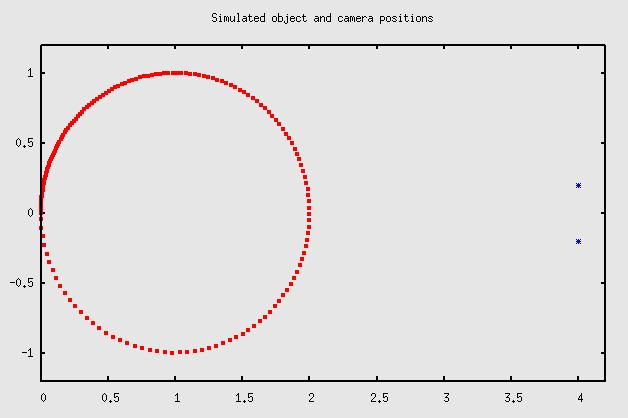
\includegraphics[width=4in]{simpos}
\end{center}

\end{frame}

%--------------------------------------------------------------------
\begin{frame}
\frametitle{Extended Kalman filter}
\framesubtitle{EKF example: simulation}

\begin{center}
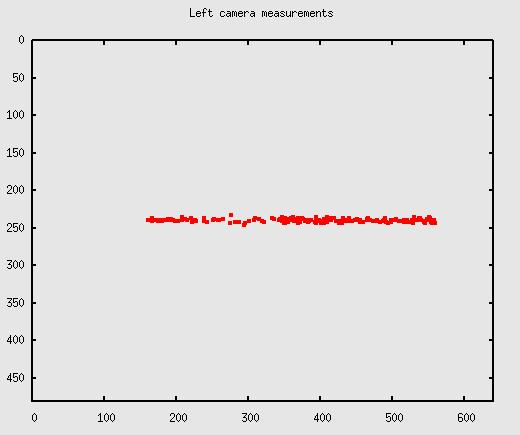
\includegraphics[width=3.5in]{left-cam}
\end{center}

\end{frame}
%--------------------------------------------------------------------
\begin{frame}
\frametitle{Extended Kalman filter}
\framesubtitle{EKF example: simulation}

\begin{center}
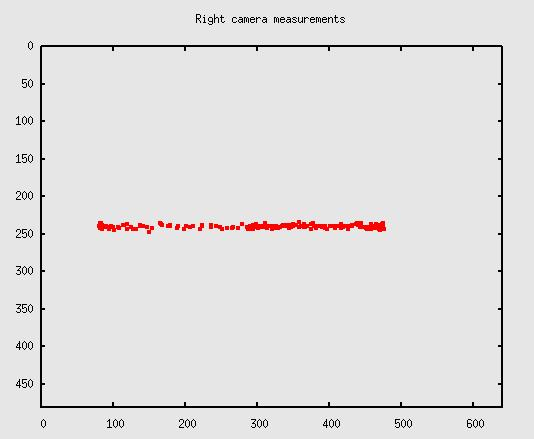
\includegraphics[width=3.5in]{right-cam}
\end{center}

\end{frame}

%--------------------------------------------------------------------
\begin{frame}
\frametitle{Extended Kalman filter}
\framesubtitle{EKF example: simulation}
\begin{center}
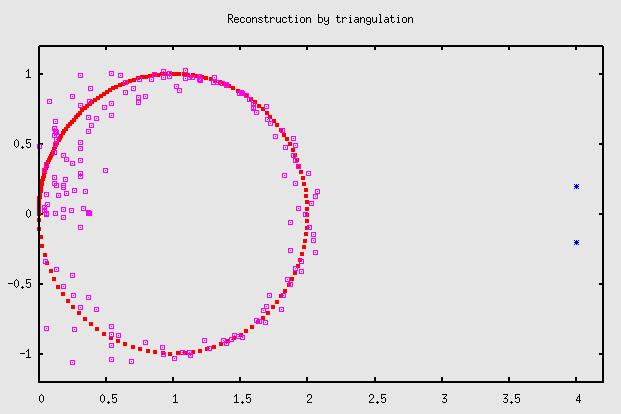
\includegraphics[width=4in]{triangulate}
\end{center}
\end{frame}

%--------------------------------------------------------------------
\begin{frame}
\frametitle{Extended Kalman filter}
\framesubtitle{EKF example: Jacobians}
Let $\vec{f}(\vec{x}) = ( f_1(\vec{x}), f_2(\vec{x}), \ldots,
f_p(\vec{x}) )^T$.

\begin{columns}
\column{3cm}
\begin{equation*}
\mat{J}_f = \begin{bmatrix} \nabla f_1(\vec{x})^T \\
\nabla f_2(\vec{x})^T \\ \ldots \\ \nabla f_p(\vec{x})^T \end{bmatrix}
\end{equation*}

\column{5cm}
\begin{equation*} \nabla f_1(\vec{x}) =
\begin{pmatrix} 1 \\ 0 \\ 0 \\
 -\Delta_t v \cos(\theta) \sin(\phi) \\ -\Delta_t v \cos(\phi)
  \sin(\theta) \\ \Delta_t \cos(\phi) \cos(\theta)
\end{pmatrix} \end{equation*}
\end{columns}

\medskip
$\nabla f_2(\vec{x}) = $ ??

$\ldots$

\medskip
$\nabla h_1(\vec{x}) = $ ??

$\ldots$

\medskip

\alert{[SHOW DEMO]}

\end{frame}

%--------------------------------------------------------------------
\section{Visual SLAM}
%--------------------------------------------------------------------

\begin{frame}
\frametitle{Visual SLAM}
\framesubtitle{Machine vision's importance for robotics}

\begin{columns}

\column{3in}

As sensors for mobile robot perception, cameras are
\begin{itemize}
\item cheap
\item small
\item lightweight
\item rich in information
\end{itemize}

\column{1.2in}

\myfig{1in}{eye}{http://www.psychol.\\cam.ac.uk}

\end{columns}

\medskip

\begin{columns}

\column{5in}

Vision facilitates \alert{interaction} with a world of objects built
for things that have eyes.

\medskip

Even the most trivial \alert{intelligent behavior} often requires
visual perception.

\end{columns}

\end{frame}


\begin{frame}
\frametitle{Visual SLAM}
\framesubtitle{But vision is hard}

When Stanford AI researchers began developing robots, \alert{planning} was
thought to be the exciting problem and \alert{perception} was at first
thought to be necessary, but easy and uninteresting.

\medskip

Vision is \alert{effortless} for us but planning sequential actions requires
\alert{conscious effort}.  Shouldn't it be the same for machines?

\medskip

In fact, AI made fast progress in planning but excruciatingly slow progress
in machine vision.

\medskip

\alert{[Show Shakey video]}

\end{frame}


\begin{frame}
\frametitle{Visual SLAM}
\framesubtitle{Two perceptual tasks for mobile robots}

In this talk we consider two problems for mobile robots:
\begin{itemize}
\item \alert{Localization}: knowing \alert{where} you are
\item \alert{Mapping}: building a model of \alert{what} (obstacles,
        objects to be manipulated) is around you
\end{itemize}

\medskip

Localization is (relatively) easy when we have an \alert{a priori map}
(build a Kalman filter or particle filter over $SE(3)$).

\medskip

Mapping is (relatively) easy when we have \alert{perfect knowledge of the
robot's locations}.

\medskip

If we don't have an a priori map, we have to build the map as we
navigate.  This is called \alert{SLAM}...


\end{frame}


\begin{frame}
\frametitle{Visual SLAM}
\framesubtitle{SLAM}

In simultaneous localization and mapping (SLAM), a robot must
\alert{map} its environment while \alert{navigating} through that
environment.

\medskip

\myfig{3in}{SLAM-Cartoon}{}

\alert{Noise}, in both the perceptual sensors and the positioning
sensors, conspires to make the task doubly difficult.

\end{frame}


\begin{frame}
\frametitle{Visual SLAM}
\framesubtitle{Applications}

\begin{columns}
\column{2.2in}

Some important applications requiring mapping and navigation:
\vspace{-0.2in}
\begin{itemize}
\item Intelligent vehicles
\item In-home assistance for the elderly and disabled
\item Medical tele-presence
\end{itemize}

\medskip

\myfig{1.5in}{figs/PR2-large}{UC Berkeley (2010)}

\column{2in}

\myfig{1.5in}{figs/the-google-car}{Google driverless car (2012)}

\medskip

\myfig{1.0in}{figs/wheelchair}{Satoh and Sakaue (2007)}

\end{columns}

\end{frame}


\begin{frame}
\frametitle{Visual SLAM}
\framesubtitle{Applications}

\begin{columns}
\column{2.0in}

More applications:
\begin{itemize}
\item Agricultural automation
\item Search and rescue
\item Surveillance and security
\item Home automation
\end{itemize}

\medskip

\myfig{2in}{figs/mower}{Husqvarna automower~(2007)}

\column{2in}

\myfig{1.5in}{figs/Orange_Harvester_Front}{Vision Robotics Corp.~(2007)}

\medskip

\myfig{1.5in}{figs/rescue-robot-19711}{Rescue Robot, NIST (2007)}

\end{columns}

\end{frame}

%--------------------------------------------------------------------
\section{Formulation}
%--------------------------------------------------------------------

\begin{frame}
\frametitle{Formulation}
\framesubtitle{Brief history}

Brief history of the most important inference tools:

\begin{itemize}
\item 1990: Stochastic map (Smith, Self, and Cheeseman)
\item 1997: Pose graphs (Lu and Milios)
\item 1998: Condensation (Isard and Blake)
\item 1999: Rao-Blackwellized particle filter (RBPF, Murphy)
\end{itemize}

\end{frame}


\begin{frame}
\frametitle{Formulation}
\framesubtitle{Formal definition of localization and mapping problems}

First, let's look at SLAM from a formal point of view.  We have a sequence
\begin{equation*}
\vec{z}_0,\vec{u}_1,\vec{z}_1,\ldots,\vec{u}_t,\vec{z}_t,\ldots,\vec{u}_T,
    \vec{z}_T,
\end{equation*}
where $\vec{z}_t$ are \alert{observations} from our sensors and
$\vec{u}_t$ represent \alert{controls} we send to the robot (wheel
encoder or accelerometer integration from $t-1$ to $t$).

\medskip

Our task is to estimate, at each point $t$ in time, a \alert{posterior
distribution}
\begin{equation*}
p(\vec{s}_t, \Theta \mid \vec{z}_{0:t}, \vec{u}_{1:t})
\end{equation*}
over the current robot \alert{location} $\vec{s}_t$ and \alert{map}
$\Theta$.

\end{frame}

\begin{frame}
\frametitle{Formulation}
\framesubtitle{Formal definition of localization and mapping problems}

Note that the
best estimates of the robot's position and map as of time $t$
would simply
be the $\vec{s}_t$ and $\Theta$ that \alert{maximize}
$p(\vec{s}_t, \Theta \mid \vec{z}_{0:t}, \vec{u}_{1:t})$.

\medskip

Note also that if the map is given and we \alert{only need to localize},
     we simply
have the special case of estimating/maximizing
\begin{equation*}
p(\vec{s}_t \mid \Theta, \vec{z}_{0:t}, \vec{u}_{1:t}),
\end{equation*}
and if the positions are given and we \alert{only need to map}, we simply
have the special case of estimating/maximizing
\begin{equation*}
p(\Theta \mid \vec{s}_{1:t} \vec{z}_{0:t}).
\end{equation*}

\end{frame}

\begin{frame}
\frametitle{Formulation}
\framesubtitle{Statistical structure}

When the dynamical system's \alert{state dynamics are Markovian} and the
\alert{observations are conditionally
independent given the state}, we obtain the dynamic Bayesian network

\myfig{2.8in}{figs/dynamical-system}{}

\vspace{-0.2in}

How does this help? Try factoring and simplifying the joint
distribution $p(\vec{s}_0, \ldots, \vec{s}_T)$.

\end{frame}


\begin{frame}
\frametitle{Formulation}
\framesubtitle{Bayes filtering}

In most cases, we want an \alert{up-to-date} estimate of the posterior
at each point $t$ in time.

\medskip

We can then recursively estimate the state using
the \alert{Bayes filter} equation

\begin{eqnarray*}
p(\vec{s}_t, \Theta \mid \vec{z}_{0:t}, \vec{u}_{1:t})
   &=& \eta \; p(\vec{z}_t \mid \vec{s}_t, \vec{\theta}_{n_t}) \\
   & & \int p(\vec{s}_t \mid \vec{s}_{t-1}, \vec{u}_t) \;
   p(\vec{s}_{t-1}, \Theta \mid \vec{z}_{0:t-1},
                \vec{u}_{1:t-1}) \; d\vec{s}_{t-1}.
   %%% \; \: \, \! are thick, medium, thin, negative thin spaces, respectively.
\end{eqnarray*}

\medskip

The three densities on the right hand side of the equation are the
\alert{sensor model}, the \alert{motion model}, and the posterior
estimate from time $t-1$.

% Would be nice to put a schematic of the HMM Bayes net here.

\end{frame}

\begin{frame}
\frametitle{Formulation}
\framesubtitle{Bayes filtering}

For clarity, suppose there is only \alert{one landmark}
observed at each point
in time (the generalization to multiple observations is straightforward).

\medskip

Then the (usually nonlinear) dynamical system can be written
\begin{eqnarray*}
  \vec{z}_t &=&
    \vec{g}(\vec{\theta}_{n_t}, \vec{s}_t) + \vec{\epsilon}_t
      \text{ (the \alert{sensor model})}\\
  \vec{s}_t &=&
    \vec{h}(\vec{s}_{t-1}, \vec{u}_t) + \vec{\delta}_t
      \text{ (the \alert{motion model})},
\end{eqnarray*}
where $n_t$ represents the index of the element $\vec{\theta}_{n_t}$ of
$\Theta$ observed at time $t$, and 
$\vec{\epsilon}_t$ and $\vec{\delta}_t$ represent the sensor noise and
odometry noise at time $t$.

\end{frame}


\begin{frame}
\frametitle{Formulation}
\framesubtitle{The EKF/stochastic map approach}

If the sensor noise and motion noise are assumed \alert{Gaussian} and
we \alert{linearize} $\vec{g}()$ and $\vec{h}()$, we obtain
the \alert{extended Kalman filter} or \alert{stochastic map} approach
proposed by Smith, Self, and Cheeseman (1990).

\medskip

But consider how the state vector grows over time.

\end{frame}


\begin{frame}
\frametitle{Formulation}
\framesubtitle{The particle filter approach}

When the noise is not well-approximated by Gaussians: we can represent
the posterior by a discrete set of \alert{samples} or
\alert{particles}.

\medskip

Particle filter approaches to SLAM differ on how the map $\Theta$ is
estimated:
\begin{itemize}
\item Some methods simply maintain a single maximum likelihood map estimate;
\item Others use the Rao-Blackewellised particle filter (RBPF, Murphy,
        1999), which maintains a \alert{different map} estimate \alert{for
    each sampled robot path}.
\end{itemize}

The RBPF is optimal, but maintaining many separate estimates of $\Theta$ is
expensive.

\end{frame}


\begin{frame}
\frametitle{Formulation}
\framesubtitle{Map representations}

The map $\Theta$ is normally represented as a 2D or 3D \alert{occupancy grid}
(Elfes, 1987) or a set of \alert{landmarks} (geometric primitives such as
points, lines, or surfaces, possibly annotated with appearance information).

\medskip

``Smarter'' maps containing \alert{surface models} or \alert{pose and
  identities of relevant objects} are also possible but less explored.

\medskip

If we're talking about visual sensors, we haven't gotten far beyond
the \alert{3D point cloud} representation.

\medskip

The RBPF has been found to work well with 2D grids and high-level
landmark lists but not with 3D grids or 3D point clouds.

\bigskip

We now vision-based SLAM specifically, where we need a 3D grid or
3D point cloud.

\end{frame}


%--------------------------------------------------------------------
\section{Mapping with stereo vision and occupancy grids}
%--------------------------------------------------------------------

\begin{frame}
\frametitle{Mapping with stereo vision and occupancy grids}
\framesubtitle{3D indoor mapping}

\begin{columns}

\column{2.5in}

A prototype autonomous vacuum cleaner built at Vision Robotics
Corp.\ in the early 2000s used
\begin{itemize}
\item Stereo vision
\item A 3D occupancy grid
\item A particle filter for robot position with the maximum likelihood
  map estimate.
\end{itemize}

\medskip

\alert{[SHOW VIDEO]}

\column{2in}

\myfig{2in}{figs/vrc-prototype}{Vision Robotics Corp.\ (2004)}

\end{columns}

\end{frame}


\begin{frame}
\frametitle{Mapping with stereo vision and occupancy grids}
\framesubtitle{2D outdoor mapping}

\begin{columns}

  \column{2in}
  
  There was some success in outdoor terrain mapping with 2D occupancy
  grids for \alert{Mars rovers} with \alert{stereo vision} (Se et al.,
  2006; Marks et al., 2008).

  \column{2.5in}
  
  \myfig{2in}{figs/Marks-Rover}{Marks, Howard, Bajracharya,
    Cottrell,\\ and Matthies (2008)}

\end{columns}

\end{frame}


\begin{frame}
\frametitle{Mapping with stereo vision and occupancy grids}
\framesubtitle{Occupancy grids}

Benefits of the occupancy grid approach:
\begin{itemize}
\item Sensor model is straightforward
\item Data association is simple
\item Robust to noisy observations
\item Good for visualization
\end{itemize}

\medskip

Disadvantages of occupancy grids:
\begin{itemize}
\item 2D grids are only sufficient for simple scenes
\item Detailed 3D grids are impractical for large-scale scenes
\item Absence of evidence is not always evidence of absence: 3D grids
  tend to provide noisy wireframe reconstructions of the scene.
\end{itemize}

\medskip

In 2020, most state-of-the-art methods use the \alert{pose graph}
approach or a variant.

\end{frame}

%--------------------------------------------------------------------
\section{Pose graph approaches}
%--------------------------------------------------------------------

\begin{frame}{Pose graph approaches}{Sparse vs.\ dense}

  We saw that occupancy grids give a \alert{dense} representation
  of the scene but have not seen much success in 3D visual mapping.

  \medskip

  There are alternative approaches to dense mapping, for example doing
  \alert{direct keyframe alignment} and generating a separate point
  cloud for each keyframe (see, e.g., LSD-SLAM).

  \medskip

  \alert{Sparse} approaches, however, represent the map as an explicit
  list of discrete landmarks.

  \medskip

  Sparsity allows us to trade off accuracy against time (number of
  landmarks) to obtain real-time computation on embedded systems.

  \medskip

  Modern successful sparse approaches are all based on the \alert{pose
    graph} approach.
  
\end{frame}


\begin{frame}{Pose graph approaches}{Setup}

  There are many ways of setting up the pose graph, depending on
  details of the robot, sensors, and approach to the optimization.

  \medskip

  Basic idea:
  \begin{itemize}
  \item \alert{Each pose} $\vec{s}_t$ is represented by \alert{one
    vertex} of the pose graph.
  \item \alert{Each landmark} $\vec{X}_i$ is represented by \alert{one
    vertex} of the pose graph.
  \item Edges connecting $\vec{s}_{t-1}$ and $\vec{s}_t$ are annotated
    with corresponding \alert{controls} $\vec{u}_t$ as constraints.
  \item Edges connecting $\vec{s}_t$ and $\vec{X}_i$ represent
    \alert{observations} $\vec{z}_{tj}$.
  \end{itemize}

\end{frame}


\begin{frame}{Pose graph approaches}{Pose graphs and graph-based optimization}

  \begin{columns}

    \column{2.3in}

    \myfig{2.0in}{kummerle-fig1}{K\"{u}mmerle et al.\ (2011), Fig.\ 1}

    \column{2.2in}

    Victoria Park dataset with unoptimized trajectory and optimized
    trajectory.

    \medskip

    Multi-level parking garage pose graph before and after
    optimization.

    \medskip

    Two views of Venice dataset after optimization.

  \end{columns}

\end{frame}


\begin{frame}{Pose graph approaches}{Setup}

  To be estimated:
  \begin{itemize}
  \item For pose vertices, we want to estimate the homogeneous
    transformation from the world frame to the body frame at time $t$
    $$\mathtt{T}_t = 
    \begin{bmatrix} \mathtt{R}_{t} & \vec{t}_{t} \\ \vec{0}^{\top} & 1 \end{bmatrix} \in SE(3)$$
    or, equivalently, $\vec{s}_t = \exp(\mathtt{T}_t) \in \lse(3)$.
  \item For landmark vertices, assuming a point cloud, we want
    to estimate $\vec{X}_i \in \Rset^3$.
  \end{itemize}
  
\end{frame}


\begin{frame}{Pose graph approaches}{An aside: Lie groups}

A Lie group $G$ comprises a smooth differentiable manifold and a group.

\medskip

In computer vision, for the group, we only care about real matrix groups
represented in $\Rset_{n\times n}$.

\medskip

The multiplication and inversion operations are the usual matrix multiplication
and matrix inversion operations.

\medskip

The group is represented by a specific sublass of $n\times n$ matrices, so
there are fewer than $n^2$ degrees of freedom.

\medskip

Elements on the differential manifold are represented by vectors in $\Rset^k$,
the number of degrees of freedom in the group.

\medskip

The $\exp()$ function maps members of the group to points on the manifold,
and the $\log()$ function does the reverse.

\end{frame}


\begin{frame}{Pose graph approaches}{An aside: Lie groups}

  See \url{https://arxiv.org/pdf/1812.01537.pdf} (\textit{A Micro Lie
    Theory for State Estimation in Robotics}, Sola et al., 2019) for a
  good summary of Lie theory for robotics.

  \medskip
  
  The most difficult-to-understand Lie algebra concept used in
  robotics is the representatio of rotations.

  \medskip

  Consider $\mat{R}(t)$ varying over time.  Clearly, $\dot{\mat{R}} =
  \frac{\partial \mat{R}}{\partial t}$ will always lie in the space
  \alert{tangent} to the manifold of valid rotation matrices.
  
  \medskip

  Rotations: 

\end{frame}


\begin{frame}{Pose graph approaches}{An aside: Lie groups}

\begin{columns}

\column{3.3in}

Performing optimization over the Lie group for 3D rotations $\lso(3)$
or 3D rigid motion $\lse(3)$ gives a minimal 3-element representation
of rotations without the \alert{gimbal lock} problem present in Euler
angle representations.

\column{2in}

\myfig{1.7in}{gimbal-lock}{From Wikipedia, \textit{Gimbal Lock}}

\end{columns}

\end{frame}


\begin{frame}{Pose graph approaches}{Setup}

  Graph optimization reduces the global optimization to a series
  of small local optimizations.

  \medskip
  
  To find a maximum likelihood estimate of $\vec{s}_t$ holding all
  other variables constant, we can assume Gaussian errors and find
  $\mathtt{T}_t$ minimizing
  \begin{itemize}
  \item The deviation $\| \vec{u}_t -
    \exp(\mathtt{T}_t\mathtt{T}_{t-1}^{-1}) \|_{\mathtt{\Sigma}_u}$
  \item The deviation $\| \vec{z}_t -
    \pi(\phi_t(\mathtt{X}),\mathtt{T}_t) \|_{\mathtt{\Sigma}_z}$,
    where $\phi_t(\cdot)$ selects the landmarks from the global
    landmark database $\mathtt{X}$ that are observed at time $t$, and
    $\pi(\cdot,\cdot)$ projects a set of 3D points into the image
    plane.
  \end{itemize}

  \medskip
  
  We begin with the guess $\mathtt{T}_t =
  \log(\vec{u}_t)\mathtt{T}_{t-1}$ then use Levenberg-Marquardt to find
  the local minimum.

  \medskip

  Estimating $\vec{X}_j$ is similar, with an initial guess from
  triangulation from two views.
  
\end{frame}


\begin{frame}{Pose graph approaches}{Implementation}

  \alert{\texttt{g2o}} (Kuemmerle et al., 2011), is probably the most
  famous toolbox for implementing graph optimization.

  \medskip

  A clean API is used to add vertices and edges run the optimization,
  and retrieve the resulting estimates.

  \medskip

  The optimizer is very lightweight and efficient, yet it is general,
  working for many different optimization problems, not only SLAM.

  \medskip

  \url{https://github.com/RainerKuemmerle/g2o}
  
\end{frame}

%--------------------------------------------------------------------
\section{LSD SLAM}
%--------------------------------------------------------------------

\begin{frame}
\frametitle{LSD SLAM}
\framesubtitle{Introduction}

Engel, St\"{u}ckler, and Cremers' (2015) method \alert{LSD SLAM}
(Large-Scale Direct) is among the best modern monocolar SLAM
methods.

\myfig{4in}{engel-fig1}{Sample LSD-SLAM results (Engel, Sch\"{o}ps,
  and Cremers, 2014)}

\end{frame}


\begin{frame}{LSD SLAM}{Principles}

  LSD-SLAM principles:
  \begin{itemize}
  \item Attempt to use all information in the image (not just
    features).
  \item Extract a series of ``keyframes'' from the video stream and
    find relationship between each pair of camera poses using graph
    optimization.
  \item Pairwise optimization in the pose graph minimizes
    \alert{photometric error} between two keyframes.
  \item Each keyframes is paired with an \alert{inverse depth map}
    containing a mean and variance (inverse confidence) in the inverse
    depth at each pixel.
  \end{itemize}

\end{frame}


\begin{frame}{LSD SLAM}{Direct vs.\ feature based methods} 

  Most SfM methods are \alert{feature based}.

  \medskip

  They first estimate camera positions and 3D point positions using
  sparse feature extraction, factorization of $\mat{E}$, resectioning,
  and bundle adjustment.

  \medskip

  A dense model can then be made through mesh construction and texture
  mapping.

  \medskip

  \alert{Direct methods} scrunch the 2-step process, finding the
  camera poses and depth maps that align images directly without
  feature extraction.
  
\end{frame}


\begin{frame}{LSD SLAM}{Notation and representation of poses}

  Camera must be \alert{calibrated} a priori.

  \medskip

  All image points are converted to
  \alert{normalized camera coordinates}
  (undistorting and multiplying by $\mat{K}^{-1}$).

  \medskip

  Instead of representing camera poses by a rotation matrix
  and translation vector packed into a 4$\times$4 homography matrix,
  we use elements of the Lie group $\lse(3)$,
  written as \alert{6-element vectors}.

  \medskip

  Similarity transformations, normally represented by a scalar scale
  factor, a rotation matrix, and a translation vector, are instead
  represented by elements of $\lsim(3)$, written as \alert{7-element
    vectors}.

\end{frame}


\begin{frame}{LSD SLAM}{Image alignment}

  Images are aligned by minimization of \alert{photometric error}
  $$E(\vec{\xi}) = \sum_i(I_{\textrm{ref}}(\vec{p}_i) - I(\omega(\vec{p}_i,
  D_{\textrm{ref}}(\vec{p}_i), \vec{\xi})))^2$$

  where
  \begin{itemize}
    \item $I(\vec{p})$ is the intensity of image $I$ at location $\vec{p}$,
    \item $\vec{\xi}$ is a possible transformation between the cameras
      imaging $I_{\textrm{ref}}$ and $I$,
    \item $\omega(\vec{p},d,\vec{\xi})$
      projects point $\vec{p}$ with inverse depth $d$ in the reference
      camera's frame into the transformed camera frame,
    \item $D_{\textrm{ref}}(\vec{p})$ is the inverse depth of 2D point
      $\vec{p}$.
  \end{itemize}

  The parameters of $\vec{\xi}$ can be estimated using an initial
  guess and Gauss-Newton minimization.
  
\end{frame}


\begin{frame}{LSD SLAM}{Outlier handling}

  Occlusions, reflections, and moving objects would introduce \alert{outliers}.

  \medskip

  Rather than remove outliers explicitly, we re-weight each point
  $\vec{p}_i$ on each iteration, down-weighting large residual errors:
  $$E(\vec{\xi}) = \sum_i w_i(\vec{\xi}) (I_{\textrm{ref}}(\vec{p}_i) - I(\omega(\vec{p}_i,
  D_{\textrm{ref}}(\vec{p}_i), \vec{\xi})))^2.$$

  Defining $r_i(\vec{\xi})$ to be the residual
  $I_{\textrm{ref}}(\vec{p}_i) - I(\omega(\vec{p}_i,
  D_{\textrm{ref}}(\vec{p}_i), \vec{\xi}))$, the Gauss-Newton update
  becomes
  $$\delta \vec{\xi}^{(n)} =
  -(\mat{J}^T\mat{W}\mat{J})^{-1}\mat{J}^T\mat{W}r(\vec{\xi}^{(n)}),$$
  where $\mat{J}$ is the Jacobian of the residuals $r_i$ with respect
  to the changes in $\vec{\xi}$.

\end{frame}


\begin{frame}{LSD SLAM}{Overview}

  Overview of the processing pipeline:

  \myfig{4.5in}{engel-fig3}{Overall LSD-SLAM flow (Engel, Sch\"{o}ps, and
    Cremers, 2014)}

\end{frame}


\begin{frame}{LSD SLAM}{Initialization}

  We begin with an initial keyframe with a \alert{random} depth map
  and a large variance.

  \medskip

  Early translations of the camera enable covergence to a nearly
  correct depth map.

\end{frame}


\begin{frame}{LSD SLAM}{Map}

  The map is a \alert{pose graph} of keyframes.

  \medskip

  \alert{Keyframe} ${\cal K}_i$:
  \begin{itemize}
  \item Image $I_i : \Omega_i \rightarrow \Rset$
  \item Inverse depth map $D_i : \Omega_{D_i} \rightarrow \Rset^+$
  \item Variance of the inverse depth $V_i : \Omega_{D_i} \rightarrow \Rset^+$
  \end{itemize}

  The depth map and variance are only defined for a subset of all
  pixels $\Omega_{D_i} \subset \Omega_i$ that have sufficient
  intensity gradient.

  \medskip

  \alert{Edges} $\xi_{ji}$:
  \begin{itemize}
  \item Similarity transform $\vec{\xi}_{ji} \in \lsim(3)$
  \item Covariance $\Sigma_{ji}$ over $\vec{\xi}_{ji}$
  \end{itemize}

\end{frame}


\begin{frame}{LSD SLAM}{Depth estimation}

  Initial $D$ starts out undefined for points with small gradient
  (purple color) and random with high variance for points with
  sufficient gradient.

  \medskip

  Camera rotation gives no additional depth information; translation
  increases confidence/decreases variance for points with parallax
  under the translation.
  
  \medskip

  \myfig{4.5in}{engel-fig4}{Inverse depth map over camera
    tranformations (Engel, Sch\"{o}ps, and Cremers, 2014).}
  
\end{frame}


\begin{frame}{LSD SLAM}{Short-term tracking}

  From each keyframe, we perform short-term tracking, finding the
  relative pose $\vec{\xi}_{ji} \in \lse(3)$ minimizing the
  \alert{robust normalized photometric resiudual}
  $$ E_p(\vec{\xi}_{ji}) = \sum_{\vec{p}\in \Omega_{D_i}} \left\|
  \frac{r^2_p(\vec{p},\vec{\xi}_{ji})}{\sigma^2_{r_p(\vec{p},\vec{\xi}_{ji})}}
  \right\|_\delta$$ where $\|\cdot\|_\delta$ is a robust norm and
  $\sigma^2_{r_p(\vec{p},\vec{\xi}_{ji})}$ is an estimate of residual
  uncertainty based on depth map uncertainty $V_i(\vec{p})$ and
  assumed constant image intensity noise $\sigma_I$.
  
\end{frame}


\begin{frame}{LSD SLAM}{New keyframes}

  A new keyframe is created from the most recent tracked image when
  the local motion $\vec{\xi}_{ji}$ exceeds a threshold.

  \medskip

  Since actual depths are unknown, the depth map for each keyframe is
  scaled so that the mean inverse depth is 1.

  \medskip

  The inverse depth map for the current keyframe is updated using the
  motion for each new tracking frame.

  \medskip

  Each new keyframe is aligned with the previous keyframe to minimize
  both photometric residual and depth residual using image
  alignment over $\lsim(3)$ --- we explicitly calculate the
  \alert{relative depth} between keyframes.

\end{frame}


\begin{frame}{LSD SLAM}{Keyframe alignment}

  \myfig{4.5in}{engel-fig5}{Direct keyframe alignment on $\lsim(3)$
    (Engel, Sch\"{o}ps, and Cremers, 2014)}

\end{frame}


\begin{frame}{LSD SLAM}{Loop closure}

  Each time a new keyframe is selected, we compare with the nearest 10
  keyframes looking for a \alert{loop closure}: a previous keyframe
  close enough to the current frame to create a new edge in the pose
  graph.

  \medskip

  Drift in a large loop might mean the new keyframe is too different
  from the best old keyframe for convergence.

  \medskip

  There are a few tricks that help in convergence, but one of the best
  is a \alert{course-to-fine} approach starting with downscaled 20$\times$15
  images.

  \medskip

  \alert{Pose graph optimization} runs continuously in the background.
  
\end{frame}


\begin{frame}{LSD SLAM}{Loop closure}

  \myfig{4.5in}{engel-fig7}{Loop closure}

\end{frame}


\begin{frame}{3D modeling}{LSD SLAM}

  LSD-SLAM runs in real time on smartphones in odometry-only
  configurations (no large-scale map).

  \medskip

  The full LSD-SLAM runs in real time on moderate CPUs (not requiring
  a GPU).

  \medskip

  ORB-SLAM runs faster than LSD-SLAM and gives more accurate
  trajectories. But the resulting point clouds are sparse.

  \medskip

  The near-term open problem is fast, accurate, dense 3D modeling from
  monocular cameras.

\end{frame}

%--------------------------------------------------------------------
\section{ORB SLAM}
%--------------------------------------------------------------------

\begin{frame}{ORB-SLAM}{Introduction}
  \begin{itemize}
  \item ORB-SLAM is a visual SLAM method
  \item In 2016, ORB-SLAM was introduced as one of the most versatile
    and accurate monocular SLAM methods to date.
  \item ORB-SLAM is based on the main ideas of
    \begin{itemize}
    \item Parallel tracking and mapping (PTAM) by Klein and Murray 
    \item
      Place recognition by G{\'a}lvez-L{\'o}pez and Tard{\'o}s 
    \item
      Scale-aware loop closing by Strasdat et. al 
    \item
      Covisibility information by Strasdat et. al
    \end{itemize}
  \end{itemize}
\end{frame}


\begin{frame}{ORB-SLAM}{Introduction}
ORB-SLAM's aims:
\begin{itemize}
    \item More efficient, simple and reliable system than existing
	    visual SLAM methods.
    \item Real-time operation in large-environments.
    \item Real-time loop closing based on optimization.
    \item Real-time relocalization with significant invariance to viewpoint
	    and illumination.
    \item Improving tracking robustness and enhance lifelong operation.
  \end{itemize}
\end{frame}


\begin{frame}{ORB-SLAM}{Introduction}
\begin{itemize}
  \item{
  Similar to other visual SLAM methods, ORB-SLAM needs a feature detector and descriptor to extract and match feature points from sequence of images.
  }  
\item{
ORB-SLAM needs a feature detector and descriptor that can be used in mapping, tracking, and place recognition processes at real time. 
}
\item{
ORB detector and descriptor are fast enough to compute and match features while having good invariance to viewpoint.
}
\item{
Therefore, ORB detector and descriptor are chosen for ORB-SLAM method.
}

\end{itemize}
  \end{frame}
  
\begin{frame}{ORB-SLAM}{Introduction}
 
\begin{itemize}
  
      \item{
ORB-SLAM consists of three threads working in parallel.
\begin{itemize}
    \item{
    Tracking thread
    }
    \item{
    Mapping thread
    }
    \item{
    Loop closing thread 
    }
\end{itemize}
}
\item{
    Bag of words place recognition is also an essential feature.
}
\item{
    The feature creates visual vocabulary from the keyframe it has been seen and stores in the database. If there are changes done to keyframes, the database is updated according to the changes.
}
\item{
    DBoW2 module is integrated to ORB-SLAM method for loop detection, relocalization, and keyframe culling.
}
  \end{itemize}
\end{frame}

\begin{frame}{ORB-SLAM}{Introduction}
  \begin{figure}
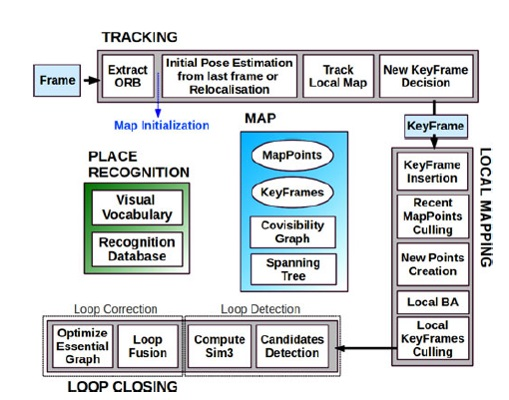
\includegraphics[scale=0.6]{figs/ORB-SLAM}
\caption{ORB-SLAM system overview}
\end{figure}
  
\end{frame}

\begin{frame}{ORB-SLAM}{Introduction}
  \begin{itemize}
      \item{
      Covisibility graph is an undirected weighted graph. Each node is a keyframe and an edge between two keyframes exists if they share observations of the same map points.
      }
      \item{
      Covisibility graph is too dense and error prone for loop closing operation. An idea of essential graph is proposed in ORB-SLAM method.
      }
      \item{
      Essential graph is a subset of covisibility graph that retains all nodes but less edges, still preserving a strong network that yields accurate results. 
      }
      \item{
      Essential graph contsins spanning trees, subsets of edges from the covisibility graph with high covisibility, and the loop closure edges, resulting in a strong network of cameras.
      }
  \end{itemize}
\end{frame}

\begin{frame}{ORB-SLAM}{Introduction}
    \begin{figure}
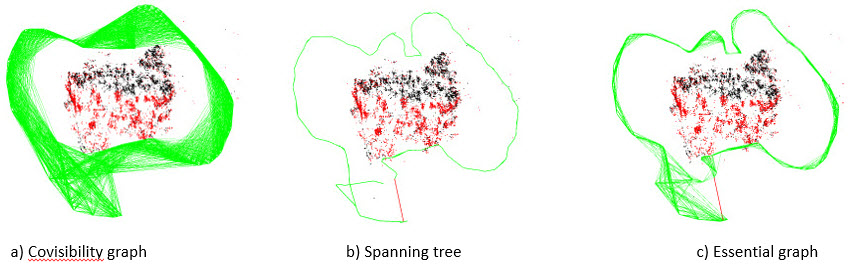
\includegraphics[scale=0.4]{figs/Graphs}
\caption{Graphs in ORB-SLAM method. a) A covisibility graph. b) A spanning tree. c) An essential graph.}
\end{figure}
  
\end{frame}

\begin{frame}{ORB-SLAM}{Tracking thread}
  \begin{itemize}
      \item{
      Tracking thread is responsible for the following tasks
      \begin{itemize}
          \item{
          Tracking       
          }
          \item{
          Map initialization
          }
          \item{
          Relocalization when tracking is lost
          }
          \item{
          Track local map
          }
          \item{
          New keyframe decision
          }
      \end{itemize}
      }
      \begin{figure}
          \centering
          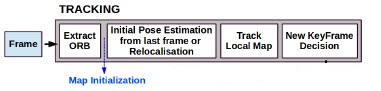
\includegraphics[scale=0.9]{figs/Tracking}
          \caption{Tracking thread overview}
      \end{figure}
      
  \end{itemize}
\end{frame}

\begin{frame}{ORB-SLAM}{Tracking thread}
    \begin{itemize}
      \item{
      Tracking thread is a process that track a set of points through successive camera frames, and using these tracks to triangulate their 3D position.
      }
      \item{
      Camera pose of each frame is estimated from the relative pose of feature points between the current frame and previous frame.
      }
      \item{
      In ORB-SLAM, tracking thread extracts and uses ORB features from every images in the video sequence.
      }  
    \end{itemize}
\end{frame}
\begin{frame}{ORB-SLAM}{Tracking thread}
\begin{figure}
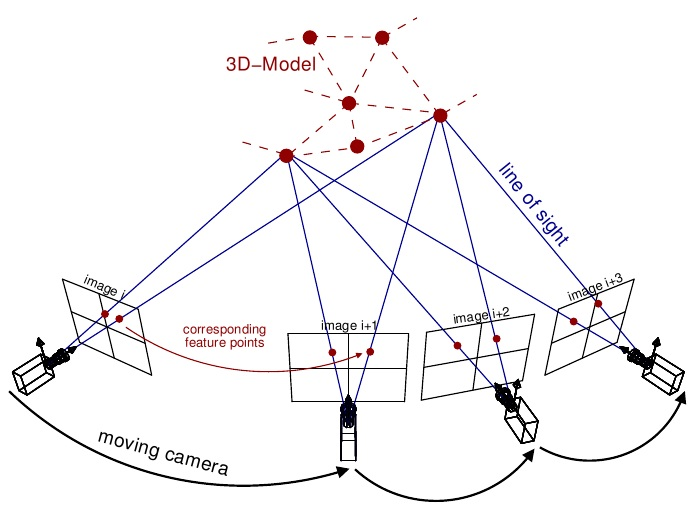
\includegraphics[scale=0.35]{figs/Triangulation}
\caption{Point triangulation. from http://www.theia-sfm.org/sfm.html}
\end{figure}
    
\end{frame}

\begin{frame}{ORB-SLAM}{Tracking thread: Map initialization}

    \begin{itemize}
    \item{
      Map initialization is the first task of the tracking thread. It triangulates initial 3D correspondences with acceptable accuracy from initial image sequences. 
      }
   \item{
   Matched features $x_{c} \leftrightarrow x_{r}$ between the current frame $f_{c}$ and the reference frame $f_{r}$ are searched to generate initial correspondences.
   }
   \item{
   Reset reference frame if not enough matches are found.
   }
   
    \end{itemize}
\end{frame}

\begin{frame}{ORB-SLAM}{Tracking thread: Map initialization}

    \begin{itemize}
    \item{
   Homography matrix $H_{cr}$ and fundamental matrix $F_{cr}$ are calculated. Tracking thread uses one of these matrices in map initialization process. 
   }
   \item{
   Homography matrix is used if the scene is planar. Fundamental matrix is selected if the scene is nonplanar. 
   }
   \item{
   The map is initialized if the selected matrix passes motion hypotheses tests and gives low reprojection error.
   }
   \item{
      Bundle adjustment is performed to refine initial correspondences and camera poses.
   }
    \end{itemize}
\end{frame}

\begin{frame}{ORB-SLAM}{Tracking thread: Map initialization}
  \begin{figure}
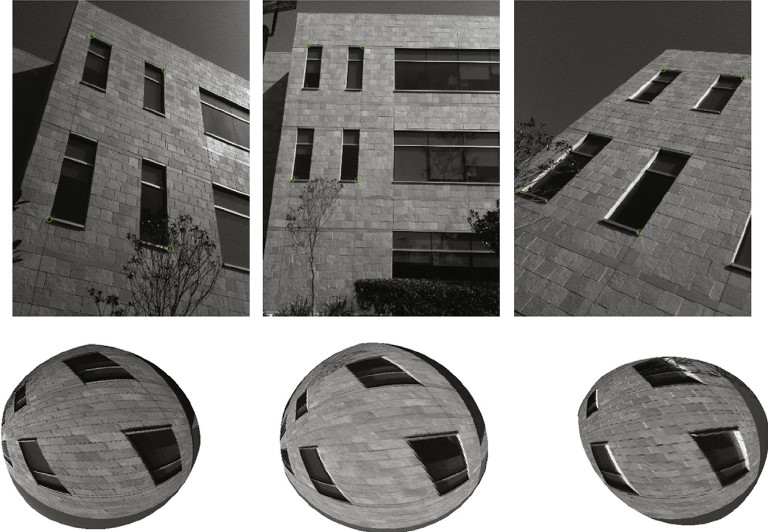
\includegraphics[scale=0.35]{figs/planar}
\caption{Different projections of a planar scene. from
  https://www.researchgate.net/figure/259128816\_fig2\_Fig-7-Digital-images-of-a-planar-scene-Top-prior-to-projective-frame-registration}
\end{figure}
\end{frame}

\begin{frame}{ORB-SLAM}{Tracking thread: Map initialization}
  \begin{figure}
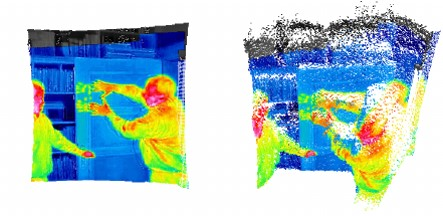
\includegraphics[scale=0.7]{figs/non_planar}
\caption{Depth maps for sample non-planar scene. from
  https://www.researchgate.net/figure/243459165\_fig15\_Figure-15-Frontal-view-onto-a-non-planar-scene-left-and-a-view-clearly-showing-the}
\end{figure}
\end{frame}

\begin{frame}{ORB-SLAM}{Tracking thread: Tracking}
  \begin{itemize}
      \item{
      Tracking continues the process from map initialization.
      }
      \item{
      If tracking was successful for last frame, camera pose in current frame is predicted with constant velocity motion model.
      }
      \item{
      If not enough matches were found, tracking thread performs wider search of the map points around their position in the last frame.
      }
      \item{
      The pose is optimized with the found correspondences.
      }
  \end{itemize}  
\end{frame}

\begin{frame}{ORB-SLAM}{Tracking thread: Relocalization}
    \begin{itemize}
        \item{
        If tracking is lost, the frame is convert into bag of words and query recognition database for keyframe candidate for global relocalization.
        }
        \item{
        Correspondences with ORB associated to map points in each key frame are computed. RANSAC iterations are performed for each keyframe to find camera pose with $PnP$ algorithm.
        }
        \item{
        If camera pose is found with enough inliers, guided search are performed to find more matches.
        }
        \item{
        The pose is then optimized and tracking procedure continues.
        }
    \end{itemize}    
\end{frame}

\begin{frame}{ORB-SLAM}{Tracking thread: Track local map}
    \begin{itemize}
        \item{
        Once estimated camera pose and an initial set of feature matches are obtained, the map into is projected to the frame and search more map point correspondences.
        }
        \item{
        The local map contains the set of keyframes $K_{1}$, that share map points with the current frame, and a set $K_{2}$ with neighbors to the keyframes $K_{1}$ in the covisibility graph.
        }
        \item{
        Map points seen in $K_{1}$ and $K_{2}$ are searched in the current frame. If found, these map points are added into the current frame and optimized.
        }
    \end{itemize}
\end{frame}

\begin{frame}{ORB-SLAM}{Tracking thread: New keyframe decision}
    \begin{itemize}
        \item{
        The current frame is verified as a keyframe if it meets the conditions
        }
        \item{
        The keyframe decided by the tracking tread is sent to the mapping thread to add into the map.
        }
        \item{
        Keyframes are inserted as fast as possible as it makes the tracking more robust to change in camera movements and rotations.
        }
        \item{
        Redundant keyframes will be culled in the mapping thread.
        }
    \end{itemize}
\end{frame}
\begin{frame}{ORB-SLAM}{Mapping thread}
    \begin{columns}[T]
\begin{column}{0.8\textwidth}
\begin{itemize}
\item{
Mapping tread is responsible for the following tasks
\begin{itemize}
    \item{
    Keyframe insertion
    }
    \item{
    Map point culling
    }
    \item{
    New map point creation
    }
    \item{
    Local bundle adjustment
    }
    \item{
    Local keyframe culling
    }
\end{itemize}
} 
\end{itemize}
\end{column}
\begin{column}{0.2\textwidth}
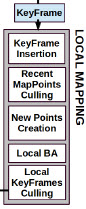
\includegraphics[width=2.5cm]{figs/localMapping}
\end{column}
\end{columns}
\end{frame}

\begin{frame}{ORB-SLAM}{Mapping thread: Keyframe insertion}
  \begin{itemize}
      \item{
      New keyframes decided by the tracking thread are added into the map.
      }
      \item{
      Nodes and edges in the covisibiilty graph are updated.
      }
      \item{
      Spanning tree and bag of word representation are updated.
      }
  \end{itemize}
\end{frame}

\begin{frame}{ORB-SLAM}{Mapping thread: Map points culling}
  \begin{itemize}
      \item{
      Map points must pass a restrictive test to ensure that they are trackable and not mistakenly triangulated.
      \begin{itemize}
          \item{
          The tracking must find the point in more than the 25 percent of the frames in which it is predicted to be visible.
          }
          \item{
          If more than one keyframe has passed from map point creation, it must be observed from at least three keyframes.
          }
      \end{itemize}
      }
  \end{itemize}
\end{frame}

\begin{frame}{ORB-SLAM}{Mapping thread: New map point creation}
    \begin{itemize}
        \item{
        For each unmatched ORB in an individual frame, unmatched correspondences are searched with other unmatched point in other keyframes.
        }
        \item{
        Newly matched map points are accepted as the new points if they pass the following tests
        \begin{itemize}
            \item{
            Positive depth test in both cameras.
            }
            \item{
            Parallax test.
            }
            \item{
            Reprojection error test.
            }
            \item{
            Scale consistency test.
            }
        \end{itemize}
        }
    \end{itemize}
\end{frame}

\begin{frame}{ORB-SLAM}{Mapping thread: Local bundle adjustment}
  \begin{itemize}
      \item{
      Local BA optimizes the currently processed keyframe ($K_{i}$), all keyframes connected to $K_{i}$ in the covisibility graph ($K_{c}$), and all map points seen by $K_{i}$ and $K_{c}$.
      }
      \item{
      Keyframes that see map points as $K_{i}$ and $K_{c}$ see are included in the optimization but remain fixed.
      }
      \item{
      Outlier are discarded in this process.
      }
  \end{itemize}
\end{frame}

\begin{frame}{ORB-SLAM}{Mapping thread: Keyframe culling}
  \begin{itemize}
      \item{
      As the complexity of bundle adjustment grows with the number of keyframes, deleting redundant keyframes benefits the system in lifelong operation.
      }
      \item{
      Keyframes that has 90 percent similar map points to its three previous keyframes are removed from the map.
      }
  \end{itemize}
\end{frame}

\begin{frame}{ORB-SLAM}{Loop closing}
  \begin{itemize}
      \item{
      Loop closing takes the last keyframe processed by the mapping thread to detect and close the loop.
      }
      \item{
      Loop closing performs the following tasks
      \begin{itemize}
          \item{
          Loop candidates detection.
          }
          \item{
          Similarity transformation estimation.
          }
          \item{
          Loop fusion.
          }
          \item{
          Essential graph optimization.
          }
      \end{itemize}
      }
  \end{itemize}
  \begin{figure}
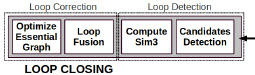
\includegraphics[scale=0.7]{figs/LoopClosing}
\caption{Loop closing overview.}
\end{figure}
\end{frame}

\begin{frame}{ORB-SLAM}{Loop closing thread: Loop candidates detection}
  \begin{itemize}
      \item{
      Similarity score is computed between the bag of word vector of the last keyframe $K_{i}$ with all of its neighbors in the covisibility graph. The lowest score $s_{min}$ is obtained.
      }
      \item{
      Recognition database is queried, keyframe whose score is lower than $s_{min}$ are not considered as loop candidates.
      }
      \item{
      All keyframes whose are directly connected to $K_{i}$ are also not considered as loop candidates.
      }
  \end{itemize}
\end{frame}

\begin{frame}{ORB-SLAM}{Loop closing thread: Similarity transformation estimation}
  \begin{itemize}
      \item{
      ORB-associated correspondences between the current keyframe and the loop candidate keyframes are calculated.
      }
      \item{
      RANSAC iterations are performed with each candidate to find a similarity transformation. 
      }
      \item{
      If the similarity is found with enough inliers, the transformation is optimized and more correspondences are searched.
      }
      \item{
      After adding more correspondences, the transformation is optimized again. If the transformation is supported by enough inliers, that loop candidate is accepted.
      }
  \end{itemize}
\end{frame}

\begin{frame}{ORB-SLAM}{Loop closing thread: Loop fusion}
  \begin{itemize}
      \item{
      Once loop closing is detected and verified, two keyframes are merged together.
      }
      \item{
      The correction for this action must be done and propagated to their neighbor keyframes in covisibility graph so they can update their proterties(i.e. recalculate transformation matrix, concatenated edges in covisibility graph). 

      }
  \end{itemize}
\end{frame}

\begin{frame}{ORB-SLAM}{Loop closing thread: Essential graph optimization}
  \begin{itemize}
      \item{
      Pose graph optimization over the Essential graph is performed to effectively close the loop.
      }
      \item{
      Scale drift is corrected, each map point is transformed according to the correction.
      }
  \end{itemize}
  
  \begin{figure}
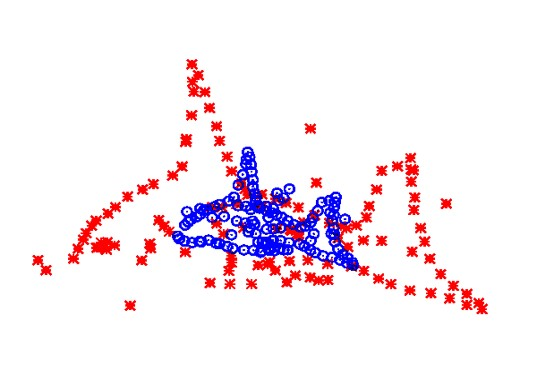
\includegraphics[scale=0.3]{figs/scaleDrift}
\caption{Scale drift.}
\end{figure}
  
\end{frame}


\begin{frame}{ORB-SLAM}{Example}
  \begin{figure}
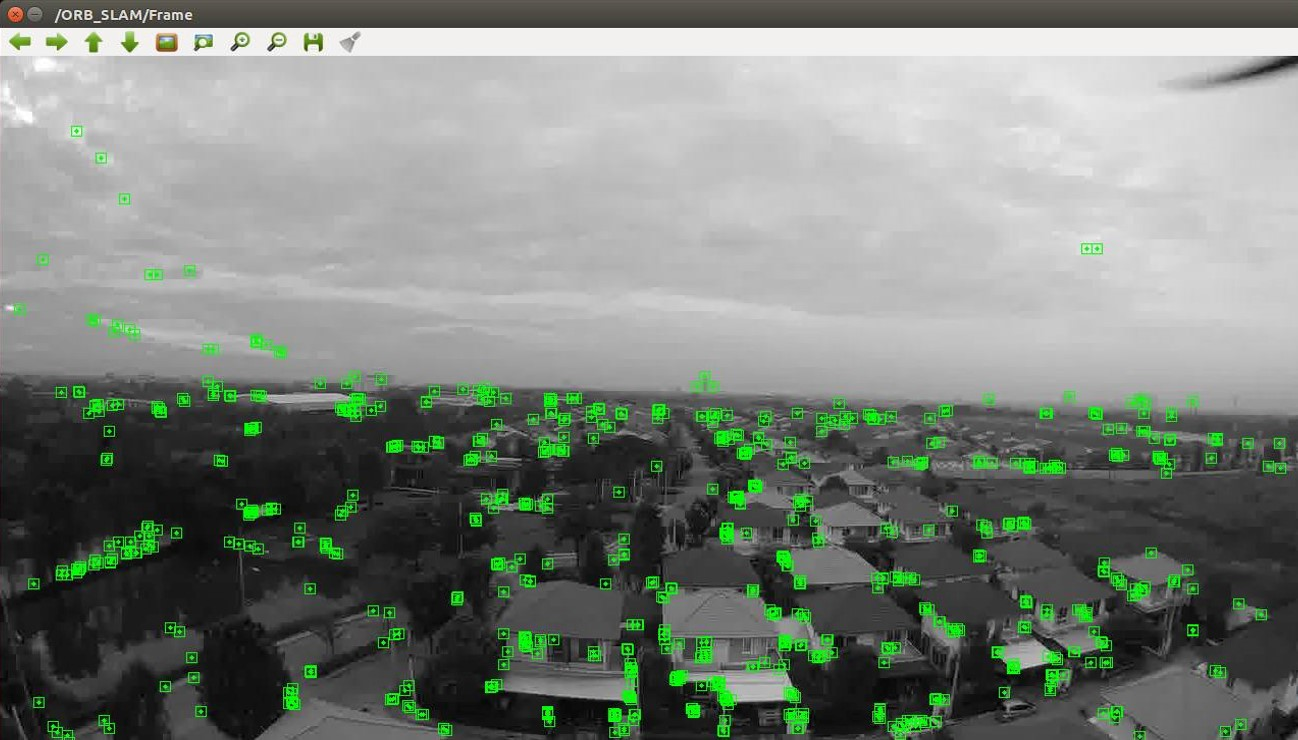
\includegraphics[scale=0.3]{figs/ORBtrack}
\caption{ORB-SLAM example: tracking.}
\end{figure}
\end{frame}

\begin{frame}{ORB-SLAM}{Example}
  \begin{figure}
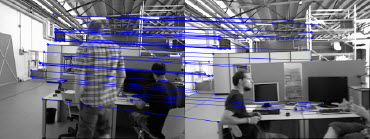
\includegraphics[scale=0.9]{figs/ORBexMapping}
\caption{ORB-SLAM example: mapping.}
\end{figure}
\end{frame}

\begin{frame}{ORB-SLAM}{Example}
  \begin{figure}
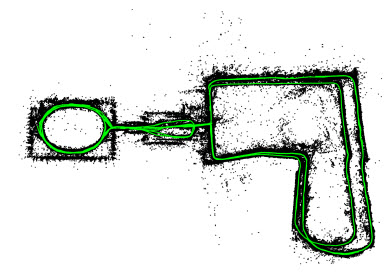
\includegraphics[scale=0.7]{figs/ORBexLoopClosing}
\caption{ORB-SLAM example: loop closing.}
\end{figure}
\end{frame}

%--------------------------------------------------------------------
\section{VI-ORB SLAM}
%--------------------------------------------------------------------

\begin{frame}{VI-ORB SLAM}{Introduction}

In 2017, the authors of ORB-SLAM
(Ra\'{u}l Mur-Artal and Juan D. Tard\'{o}s)
introduced ``Visual-Inertial Monocular SLAM with Map Reuse.''

\medskip

We know that all
monocular SLAM methods
have the limitation of \alert{scale ambiguity}.

\medskip

By adding information from GPS or an IMU, we can resolve that ambiguity.

\medskip

Existing work:
\begin{itemize}
\item IMU preintegration by Lupton and Sukkarieh (2012)
\item IMU preintegration mapped to SO(3) by Forster et al. (2016)
\item Factor graph representation by Indelman et al. (2013)
\item ORB SLAM (2016)
\end{itemize}

\end{frame}


\begin{frame}{VI-ORB SLAM}{Overview}

\begin{columns}

\column{2.5in}

\myfig{2.3in}{murartal-fig1}{Mur-Artal and Tard\'{o}s (2017), Fig.\ 1}

\column{2in}

ORB SLAM performs tracking for the current frame using a fixed map.

\medskip

On the back end, local Bundle Adjustment (BA) optimizes a local window
of keyframes.

\medskip

Large loops are detected using place recognition then corrected using
lightweight pose graph optimization followed by full BA.

\medskip

Sample result on left.

\end{columns}

\end{frame}


\begin{frame}{VI-ORB SLAM}{Avoiding biased partial solutions}

Each step (tracking and local BA) fixes some states in their optimization.

\medskip

This could bias the final solution, so it is important to get a good
start.

\medskip

To reduce any such bias, the authors implement a VI full BA that optimizes
structure, camera poses, scale, velocities, gravity, and gyroscope and
accelerometer biases.

\medskip

But BA always needs an initial guess. The authors propose a
piece-by-piece approach to obtain this solution (next slide).

\end{frame}


\begin{frame}{VI-ORB SLAM}{Avoiding biased partial solutions}

Idea of initialization:
\begin{itemize}
\item Process a few seconds of video with regular ORB SLAM. This gives an
initial solution for structure and some keyframe poses up to unknown scale.
\item Compute bias of the gyroscope based on known orientation of the keyframes.
\item Solve for scale and gravity without accelerometer bias.
\item Using knowledge of the magnitude of gravity, solve for accelerometer
bias, refining scale and gravity direction.
\item Extract velocity for each keyframe.
\end{itemize}

\medskip

The main requirement is that the sensor should be moved in such a way as
to make all variables observable.

\end{frame}


\begin{frame}{VI-ORB SLAM}{Visual-inertial odometry}

The VI odometry method is based on a few key aspects.

\medskip

We assume a \alert{pinhole camera}.
Keypoints are extracted on original image, but
coordinates are undistorted before being used.

\medskip

There is an IMU that works as follows:
\begin{itemize}
\item Acceleration $\vec{a}_b^k$ at time $k$ in the IMU frame $b$.
\item Angular velocity $\vec{\omega}_b^k$ at time $k$ in the IMU frame $b$.
\item Update frequency is on the order of 100 Hz.
\item Accelerometer modeled as having slowly varying biases
      $\vec{b}_a^k$ and $\vec{b}_g^k$
      for the accelerometer and gyroscope.
\item Accelerometer is subject to gravity $\vec{g}_w$,
      which must be subtracted in order to compute motion.
\end{itemize}

\end{frame}


\begin{frame}{VI-ORB SLAM}{Visual-inertial odometry}

Goal of the system: estimate state parameters and 3D points over time.
\begin{itemize}
\item $\mat{R}_{wb}^k$ is the
   rotation of the IMU in the world frame at time $k$.
\item $_w\vec{v}_b^{k}$
   is the velocity in the world frame at time $k$.
\item $_w\vec{p}_b^{k}$ is
   the position of the IMU in the world frame at time $k$.
\end{itemize}

\medskip

Model is as follows:

   $$\mat{R}_{wb}^{k+1} = \mat{R}_{wb}^k \exp\left((\vec{\omega}_b^k-\vec{b}_g^k)\Delta_t\right)$$

  $$_w\vec{v}_b^{k+1} =\ _w\vec{v}_b^k + \vec{g}_w \Delta_t + \mat{R}_{wb}^k(\vec{a}^k_b-\vec{b}^k_a)\Delta_t$$

  $$_w\vec{p}_b^{k+1} =\ _w\vec{p}_b^k +\ _w\vec{v}_b^k\Delta_t + \frac{1}{2}\vec{g}_w\Delta_t^2 + \frac{1}{2}\mat{R}^k_{wb}(\vec{a}_b^k-\vec{b}^k_a)\Delta_t^2$$.

\end{frame}


\begin{frame}{VI-ORB SLAM}{Visual-inertial odometry}

$\exp(\cdot)$ is ``exponential map'' of rotations, a function mapping a
twist vector $\vec{v} \in \Rset^3$
(denoting a rotation of $\|\vec{v}\|$ about the
unit vector $\vec{v}/\|\vec{v}\|$) to a rotation matrix.

\medskip

IMU measurements between two keyframes are preintegrated based on
the work of Forster et al. (2016):
   
   $$\mat{R}_{wb}^{i+1} = \mat{R}_{wb}^i\Delta_{\mat{R}_{i,i+1}}\exp(\mat{J}^g_{\Delta R}\vec{b}^i_g)$$

   $$_w\vec{v}_b^{i+1} = _w\vec{v}^i_b + \vec{g}_w\Delta_{t_{i,i+1}} +
      \mat{R}_{wb}^i(\Delta_{\vec{v}_{i,i+1}} + \mat{J}^g_{\Delta_v}\vec{b}^i_g
      + \mat{J}^a_{\Delta_{\vec{v}}}\vec{b}^i_a)$$

   $$_w\vec{p}_b^{i+1} = _w\vec{p}^i_b + \vec{v}^i_b\Delta_{t_{i,i+1}} +
      \frac{1}{2}\vec{g}_w\Delta_{t_{i,i+1}}^2 +
      \mat{R}_{wb}^i\left(\Delta_{\vec{p}_{i,i+1}} + \mat{J}^g_{\Delta_p}\vec{b}^i_g
      + \mat{J}^a_{\Delta_{\vec{p}}}\vec{b}^i_a\right)$$

\end{frame}


\begin{frame}{VI-ORB SLAM}{Visual-inertial odometry}

  The idea is to separate the effect of the bias from the pre-integrated
  IMU measurements with a linear approximation.

  \medskip

  The values $\Delta_{\mat{R}_{i,i+1}}$,
             $\Delta_{\vec{v}_{i,i+1}}$, and
             $\Delta_{\vec{p}_{i,i+1}}$ are the
  simple integration/concatenation
  of the transformations given by the IMU over the period between
  keyframe $i$ and $i+1$.
  

  The preintegrations and Jacobians are computed iteratively as the IMU
  measurements arrive.

\end{frame}


\begin{frame}{VI-ORB SLAM}{Visual-inertial odometry}

Finally, the
camera and IMU are considered rigidly attached with transformation
$$\mat{T}_{cb} = \begin{bmatrix} \mat{R}_{cb} \mid\ _c\vec{p}_b \end{bmatrix}$$
between their frames.

\medskip

The transformation is estimated from the calibration
method of Furgale et al. (2013) implemented in the open-source \alert{Kalibr}
tool.

\end{frame}


\begin{frame}{VI-ORB SLAM}{Modifying ORB-SLAM for VI odometry}

As before, ORB-SLAM has 3 parallel threads: tracking, local mapping, and loop
closing.

\medskip

For the \alert{tracking thread}:
\begin{itemize}
\item At each new frame, camera pose is predicted based on
   the IMU and the estimated pose from the previous frame.
\item Visible keypoints
   are projected to the new frame then matched.
\item Then the new frame's pose
   is optimized considering the matches and the IMU error.
\end{itemize}

\end{frame}


\begin{frame}{VI-ORB SLAM}{Modifying ORB-SLAM for VI odometry}

Main idea for tracking thread:

\medskip

\myfig{4in}{murartal-fig2}{Mur-Artal and Tard\'{o}s (2017), Fig.\ 2.}

\medskip

As long as we are tracking successfully and the local mapping thread does
not update 3D point locations, we continue to incrementally update the
pose relative to the previous keyframe.

\medskip

When the mapping thread updates
the keyframe pose, we reset the current frame's
pose relative to the keyframe that changed, then resume incremental
updates.

\end{frame}


\begin{frame}{VI-ORB SLAM}{Modifying ORB-SLAM for VI odometry}

[More on tracking thread]

\medskip

The frame-changed optimization uses the parameter vector

$$\vec{\theta} = \left\{ \mat{R}^j_{wb},_w\vec{p}_b^j,_w\vec{v}^j_b,
                         \vec{b}^j_g,\vec{b}_a^j \right\}$$

$$\vec{\theta}^* = \argmin_{\vec{\theta}} \left(\sum_k E_{\mathrm{proj}}(k,j)
                                              + E_{\mathrm{IMU}}(i,j)\right)$$

This is the sum of the reprojection error for all visible 3D points $k$
and the IMU error from keyframe $i$ to new frame $j$.

\medskip

The frame-unchanged optimization uses a joint optimization of parameters
for frame $j$ and frame $j+1$.

\end{frame}


\begin{frame}{VI-ORB SLAM}{Modifying ORB-SLAM for VI odometry}

\begin{columns}

\column{2.2in}

The \alert{local mapping thread}
performs a local BA every time a new
keyframe is inserted.

\medskip

An $N$ keyframe window is optimized with all of
the points observed over those keyframes (see right).

\medskip

ORB-SLAM merely optimizes the poses and 3D points with reprojection error
as the objective, whereas VI-ORB SLAM additionally adds IMU error terms
for velocity and biases.

\column{2.3in}

\myfig{2.0in}{murartal-fig3}{Mur-Artal and Tardo\'{o}s (2017), Fig.\ 3}

\end{columns}

\end{frame}


\begin{frame}{VI-ORB SLAM}{Modifying ORB-SLAM for VI odometry}

The \alert{loop closing thread}
tries to reduce drift when returning to an already-mapped area.

\medskip

The place recognition module matches recent keyframes with
past keyframes.

\medskip

If a rigid-body transformation can be found, then an
optimization is carried out over the whole trajectory.

\medskip

First is a pose-graph optmization that ignores IMU data, followed by a
full BA that optimizes all velocities, biases, positions, and so on.

\end{frame}


\begin{frame}{VI-ORB SLAM}{Conclusion}

Result: \alert{accurate},
\alert{real time}, \alert{sparse} solution to the
SLAM problem.

\medskip

We learn that a monocular camera with IMU (and some sophisticated
processing software) is sufficient for accurate localization
and sparse point cloud mapping in real time.

\medskip

No need for lasers, ultrasonic sensors, etc.!

\medskip

See \url{https://www.youtube.com/watch?v=rdR5OR8egGI} and other examples.

\medskip

See \url{https://github.com/jingpang/LearnVIORB} for community
implementation based on the authors' ORB-SLAM 2 implementation.

\medskip

Interesting project: get VI-ORB SLAM running on Android, using the
smartphone IMU!

\medskip

Another: compare VI-ORB-SLAM with OKVIS and SVO-2 (\url{https://www.youtube.com/watch?v=hR8uq1RTUfA&t=33s}).

\end{frame}


%--------------------------------------------------------------------
\section{Ongoing research at AIT}
%--------------------------------------------------------------------

\begin{frame}
\frametitle{Ongoing research at AIT} \framesubtitle{Current vision and
  robotics research}

Current related research in the AI Center at AIT:
\begin{itemize}
\item Mobile video processing platform for agricultural crop mapping and
  yield prediction
\item 3D virtual model construction and visualization for an agricultural 
  field inspection robot 
\item Environment modeling for a security robot
\item Local path planning and execution for mobile target pursuit robot
\item Target tracking for mobile target pursuit
\item Kinect-enabled autonomous assistant robot
\item Autonomous navigation for a quad-rotor UAV with
  monocular camera for outdoor cluttered environments
\end{itemize}

\end{frame}

\begin{frame}
\frametitle{Ongoing research at AIT}
\framesubtitle{Localization from human-made maps}

In other work, we are exploring the use of a priori maps for
vision-based localization of autonomous vehicles that also have
GPS and electronic compass sensors.

\medskip

We said that localization from an a priori map is ``easy,'' but the
map must be in a usable form.

\medskip

The idea is to combine satellite imagery with ground-based image processing
for the sensor model then fuse GPS, compass, and vision data using
the particle filter.

\end{frame}


\begin{frame}
\frametitle{Ongoing research at AIT}
\framesubtitle{Mobile video processing for agricultural crop mapping}

Current work in agricultural crop mapping:

\medskip

\myfig{4.0in}{figs/MobileRobotPlatform}{}

\end{frame}


\begin{frame}
\frametitle{Ongoing research at AIT}
\framesubtitle{Mobile video processing for agricultural crop mapping}

\myfig{4.0in}{figs/SmartPhonePlatform}{}

\end{frame}

\begin{frame}
\frametitle{Ongoing research at AIT}
\framesubtitle{Mobile video processing for agricultural crop mapping}

This project proposes a method for applying 3D reconstruction to an image sequence
to get a 3D virtual model.

\medskip
\myfig{2.5in}{figs/sequence}{Image sequence extracted from video file
taken from agricultural field}

\end{frame}


\begin{frame}
\frametitle{Ongoing research at AIT}
\framesubtitle{Mobile video processing for agricultural crop mapping}

We apply keyframe selection to the video sequence, find fruit regions,
and perform 3D reconstruction of the point regions.

\begin{columns}

\column{1.5in}
\myfig{1.5in}{figs/manual_ss5}{}
\column{1.5in}
\myfig{1.5in}{figs/manual_ss4}{}
\end{columns}

\end{frame}

\begin{frame}
\frametitle{Ongoing research at AIT}
\framesubtitle{Environment modeling for security robots}

We are working on 3D modeling of obstacles from a single camera for
purposes of robot navigation.

\medskip

Experiments on our surveillance robot use the open source ROS framework.

\begin{columns}

\column{1.2in}
\myfig{1.1in}{figs/correspond_force_straight_2}{}
\column{1.2in}
\myfig{1.1in}{figs/exp-3-force-straight}{}
\end{columns}

\end{frame}


\begin{frame}
\frametitle{Ongoing research at AIT}
\framesubtitle{Local path planning and execution for mobile target pursuit}

Here we are working on algorithms to plan local obstacle-avoidance trajectories
in order to pursue a moving target.

\medskip

\myfig{2.0in}{figs/meu3}{Example pursuit path plan}

\end{frame}


\begin{frame}
\frametitle{Ongoing research at AIT}
\framesubtitle{Target tracking for pursuit robot}

We are putting these algorithms together for
pursuit of suspicious targets using a monocular
camera mounted on a pursuit robot. 
 
\medskip

\myfig{2.5in}{figs/PursuitRobot}{Pursuit robot prototype}

\end{frame}


\begin{frame}
\frametitle{Ongoing research at AIT}
\framesubtitle{Target tracking for pursuit robot}

The operator manually specifies a target to track.

\medskip

We track the object using color histogram tracking,
a model of the robot's kinematics, a model of the target's dynamics,
and an extended Kalman filter.

\medskip

\myfig{2.0in}{figs/camera_view_with_object}{Tracking object from 
camera view in simulator}

\end{frame}


\begin{frame}
\frametitle{Ongoing research at AIT}
\framesubtitle{Target tracking for pursuit robot}

Testing is ongoing using synthetic simulations, a Gazebo simulation under
ROS, and experiments on the physical pursuit robot.

\medskip

\myfig{3.2in}{figs/ait_robot_object}{Target tracking in simulator}

\end{frame}

\begin{frame}
\frametitle{Ongoing research at AIT}
\framesubtitle{Kinect-enabled autonomous assistant robot}

This project explores the use of the Willow Garage
Turtlebot and Microsoft Kinect
to carry documents in an office or orders in a restaurant.

\medskip

Users can interact with the robot via speech, hand gestures,
      or a Web interface.

\medskip

The Robot Operating System (ROS) is the main framework.

\medskip

The Web 
interface part uses the
\texttt{rosbridge} tool to handle message passing
between ROS and JavaScript programs running in the Web browser
over a Web socket.

\end{frame}


\begin{frame}
\frametitle{Kinect-enabled autonomous assistant robot}

\myfig{4.0in}{figs/navigation_kinect_04}{Robot navigation and 
obstacle avoidance using Kinect}

\end{frame}


\begin{frame}
\frametitle{Ongoing research at AIT}
\framesubtitle{Kinect-enabled autonomous assistant robot}

\myfig{3.5in}{figs/speech_matthew}{Localization using
    Kinect and a 2D obstacle map}

\end{frame}


\begin{frame}
\frametitle{Ongoing research at AIT}
\framesubtitle{Autonomous navigation for a quad-rotor UAV}

This project uses a quad-copter with a low-resolution camera to gather
videos
of agricultural fields for inspection purposes.

\medskip

Objectives:
\begin{itemize}
\item To obtain \alert{high-resolution} image of a 3D scene using low quality,
		 low-resolution monocular camera mounted on the quad-copter.
\item To improve the quality of \alert{3D-reconstruction} by selecting key
         frames constructed using super-resolution.
\end{itemize}

\begin{columns}
\column{1.5in}
\myfig{1.5in}{figs/QuadCopter}{Quad-copter}
\column{1.5in}
\myfig{1.5in}{figs/image1249}{Image taken from quad-copter}
\end{columns}

\end{frame}


\begin{frame}
\frametitle{Ongoing research at AIT}
\framesubtitle{Autonomous navigation for a quadrotor UAV}
 
\begin{itemize}
\item We are developing simultaneous real-time navigation
  based on feature tracking and non-real-time \alert{3D reconstruction}.
\item Eventually the work will enable
  detection of weed and pest infestation using the high-resolution frames
  constructed by super-resolution.
\end{itemize}
 
\myfig{2.5in}{figs/3Dreconstruction}{3D reconstruction} 
 
\end{frame}

%--------------------------------------------------------------------
\section{Conclusion}
%--------------------------------------------------------------------

\begin{frame}
\frametitle{Conclusion}

Vision sensors are \alert{information-rich}, \alert{cheap}, and 
\alert{lightweight}.

\medskip

Using vision sensors in practical mobile robot applications requires
solutions to challenging AI problems.

\medskip

A few of the open problems:
\begin{itemize}
\item Incremental localization and mapping
  algorithms are not yet as accurate as
  batch structure-from-motion algorithms in traditional computer vision.
\item The higher level geometry of complex scenes is still not as
  accurate as we would like.
\item Current methods with current sensors and embedded processors are
  prone to lose track when motion is too large or scene texture is too
  weak.
\item What about control? Can we really use these tools to build
  obstacle maps in real time and feed the information to the control
  loop?
\end{itemize}

\end{frame}


\begin{frame}
\frametitle{Conclusion}
\framesubtitle{The big problem for AI}

\begin{block}{The big challenge for AI approaches to visual perception}
It is difficult to impose high-level top-down constraints (e.g.\ that
walls and floors are normally planar and orthogonal) on
bottom-up statistical inference algorithms.

\medskip

The field needs methods
for combining high-level knowledge representation
with low-level statistical inference!
\end{block}

\end{frame}

\end{document}

